\documentclass[PaulGanssle-Thesis.tex]{subfiles}

\begin{document}
\chapter{Relaxometry and Diffusometry}
\label{relaxometry}
\section{Overview}
\label{relaxometry.overview}
Relaxometry and diffusometry are important tools for the characterization of heterogeneous materials and porous media\cite{song-nmr-chemical-engineering-2006}, with applications including the study of biological systems,\cite{seland-mri-2005,kopf-biophys-1996} medical imaging, food characterization\cite{hurlimann-jcis-2006,guthausen-jaocs-2004} and oil-well logging.\cite{kleinberg-cmr-2001,hurlimann-emr-2012} These methods can be extremely effective in applications where high-resolution NMR is either unnecessary, impractical or both. The pulse sequences used to make these measurements are often robust even in the presence of sample motion, strong gradients and pulse imperfections,\cite{hurlimann-jmr-2000,hurlimann-jmr-2001} allowing for the use of magnetic resonance in extreme environments or under conditions with rigid design constraints. Relaxometry and diffusometry are often used when making \emph{ex-situ} measurements - wherein the geometry of the usual NMR experiment is inverted and a detector is used to either probe the surface of a larger sample or it is entirely surrounded by the sample.\cite{blumich-mri-mouse-1998,single-sided-nmr,jackson-jmr-1980} In these cases, the volume and geometry within which it is possible to create a homogeneous field are limited, and in general it is not feasible to generate the field strengths necessary to make high resolution NMR measurements; however, relaxation and diffusion depend on many environmental factors including chemical composition, pressure\cite{defries-jcp-1977}, temperature,\cite{Simpson1958,bentum-2011} phase\cite{lerumeur-mri-1987,resing-jcp-1965} and even sample geometry,\cite{vanderweerd-jmr-2002} and as such measurements of these processes can yield considerable information about the sample.

\section{Spin-Lattice Relaxation (T$_1$)}
\label{Section:Relaxometry-T1}
Spin-lattice relaxation is the mechanism by which non-equilibrium spin polarization returns to its equilibrium state by energy exchange with the environment (called the lattice). In traditional high-field experiments, this takes the form of spins tipped into a transverse plane re-aligning with the bias offset field, and would be measured using an inversion-recovery or saturation-recovery experiment. In low-field experiments, however, the initial polarization induced by the prepolarizing magnet is much higher than the endpoint polarization in small bias fields (see Sec. \ref{relaxometry.t1.uncertainty.decayendpoint} for more details), and so spin-lattice relaxation causes re-equilibration to near-zero polarization and thus represents approximately a pure loss of spin polarization.\cite{Levitt2008}

\subsection{Pulse Sequence}
\label{Section:Relaxometry-T1-PulseSequence}
\begin{figure}[ht!]
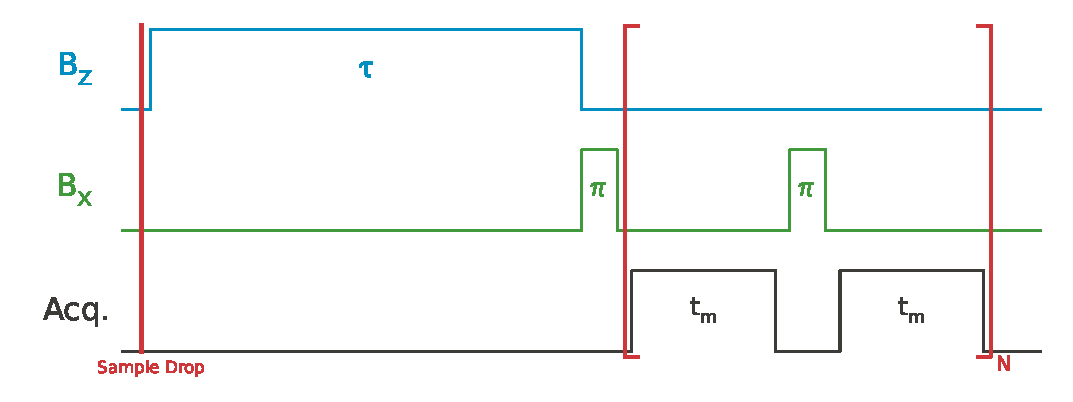
\includegraphics[width=\tw]{figures/relaxometry/t1_sequence_diagram.eps}
\caption{Pulse sequence for indirect acquisition of $\mathrm{T}_{1}$ at low field.}
\label{fig:relaxometry.t1.pulsesequence}
\end{figure}

The $\mathrm{T}_{1}$ measurement consists of prepolarizing a simple, field cycling to the desired field and after a time $\tau$ measuring the remaining spin magnetization. This is always done in an indirect dimension to allow for greater flexibility in the experimental design - the bias field ($B_z$ in Fig. \ref{fig:relaxometry.t1.pulsesequence}) can be set to an arbitrary value between $\approx$ 0 and \unit[1]{G} without the need to recalibrate pulse length or power, or to recalibrate the magnetometer.

For a prepolarizing field $B_{PP}$ and sample transit time $t_t$, the full equation for signal intensity as a function of $\tau$ is given by Eqn \ref{eqn:T1DecayFull}:

\begin{equation}
M(t) = \left[\frac{\gamma B_{PP}}{k_{B}T}e^{-\sfrac{t_t}{T_{1,t}}} + \frac{\gamma B_{tt}}{k_{B}T}\left(1-e^{-\sfrac{\tau}{T_{1,B_{Z}}}}\right)\right]e^{-\sfrac{\tau}{T_{1,B_{Z}}}} + \frac{\gamma B_{Z}}{k_{B}T}\left(1-e^{-\sfrac{\tau}{T_{1,B_{Z}}}}\right),
\label{eqn:T1DecayFull}
\end{equation}

where $\mathrm{T}_{1,B_{Z}}$ is the T$_1$ in field B$_{z}$ and T$_{1,t}$ is the effective T$_{1}$ during the shuttling period. For $B_{z}, B_{tt} \ll B_{PP}$, this simplifies to Eqn \ref{eqn:T1Decay}:

\begin{equation}
\label{eqn:T1Decay}
M(\tau) = \frac{\gamma B_{PP}}{k_{B}T}e^{-\sfrac{t_t}{T_{1,t}}}e^{-\sfrac{\tau}{T_{1,B_{Z}}}}.
\end{equation}

The results are then fit using a standard exponential $Ae^{-\sfrac{\tau}{T_1}}$, where $A$ should be constant with respect to $\tau$ (more on when this assumption breaks down in Sec. \ref{relaxometry.t1.uncertainty}).

\subsection{Temperature Dependence}
\label{relaxometry.t1.tempdependence}
The mechanisms by which spin-lattice relaxation occurs can depend on temperature, with the temperature effect being particularly pronounced in the case of water.\cite{Hindman1973} This is particularly important in these experiments, wherein the magnetometer cell is maintained at an elevated temperature. Small changes in the insulation properties of the heater or probe can lead to significant changes in the temperature of the liquid samples. Moreover, because the samples are pneumatically shuttled between the polarization and detection regions, it is very difficult to undertake in line temperature measurements during experiments.

Assuming the samples reach equilibrium sufficiently quickly (or, once reached, do not cool significantly between measurements), the temperature dependence of $\mathrm{T}_{1}$ and $\mathrm{T}_{2}$ can be used as a measure of the sample temperature. This is explored in more detail in Sec. \ref{nmr.sampletemp.relaxation}.

\subsection{Uncertainty}
\label{relaxometry.t1.uncertainty}
There are several sources of uncertainty in these relaxation measurements of varying importance. The most prominent mechanism for uncertainty is error on the measurements themselves - this is an error on the magnetization, which can be occasionally difficult to definitively characterize. Likely the most accurate way to characterize the error is by taking the standard deviation of repeated measurements, but this raises some question about what is to be considered a measurement. Magnetization measurements consist of a series of direct-dimension measurements of the magnetization, which are aggregated into a sort of average magnetization value over the direct dimension. Most forms of random noise are largely self-similar, and so the two methods of noise characterization should be roughly equivalent. However, one of the greatest difficulties in characterizing the uncertainty comes from the fact that many of the greatest sources of noise in our experiments are discrete noise, which only averages if the phase is shifting over time. For $N\rightarrow\infty$, the noise from discrete sources will converge to 0, but in the short run, the noise characteristics can be unpredictable, and there may be significant differences between the noise on each direct-dimension measurement and the noise on the cumulative measurements.

\subsubsection{Temperature uncertainty}
\label{relaxometry.t1.uncertainty.temp}
One significant potential source of uncertainty is temperature shifts. The $\mathrm{T}_{1}$ as a function of temperature is parametrized as:\cite{Hindman1973,bentum-2011,Simpson1958}

\begin{equation}
\frac{1}{T_{1}} = A_{1}\mathrm{e}^{\sfrac{E_{1}}{RT}}A_{2}\mathrm{e}^{\sfrac{E_{2}}{RT}}
\end{equation}

$E_1$ and $E_2$ are activation energies for the two contributions to the intermolecular relaxation, and our measured values of $E_{1}$ = \unitfrac[4.45$\cdot $10$^{4}$]{kJ}{mol} and $E_{2}$ = \unit[1.49$\cdot $10$^{4}$]{kJ}{mol} are in strong agreement with measurements at \unit[1.4]{T}\cite{Hindman1973} and \unit[3.4]{T}. The pre-exponential factors at \unit[0.435]{G} were found to be $A_{1}$ = \unit[1.30$\cdot $10$^{-9}$]{s} and $A_{2}$ = \unit[8.49$\cdot \mathrm{10}^{-4}$]{s}, which also has strong agreement with the higher-field experimental data. Propagating the error in $T$ gives:

\begin{equation}
\label{eqn:TError}
\sigma_{T_{1}} = \left|\frac{A_{1}E_{1}\mathrm{e}^{\sfrac{E_{1}}{RT}} + A_{2}E_{2}\mathrm{e}^{\sfrac{E_{2}}{RT}}}{RT^2\left(A_{1}\mathrm{e}^{\sfrac{E_{1}}{RT}} + A_{2}\mathrm{e}^{\sfrac{E_{2}}{RT}}\right)^2}\sigma_{T}\right|
\end{equation}

For the same reasons that it is difficult to measure the temperature in the first place, though, it is even more difficult to measure the temperature fluctuations, and so a robust measure of $\sigma_T$ cannot be made. Assuming a scenario of fluctuations on the order of $\sigma_{T}$ = \unit[2]{K} (likely the equilibrium fluctuations are smaller than this) at $\approx$ \unit[38]{K}, the error $\sigma_{T1}$ would be $\approx$ \unit[0.178]{s} (4.6\%). Even for $\sigma_{T}$ = \unit[10]{K}, the error $\sigma_{T1}$ would be \unit[0.89]{s} (20\%). Even here, temperature fluctuations will likely average out over the course of a full experiment.

\subsubsection{Decay Endpoint}
\label{relaxometry.t1.uncertainty.decayendpoint}
These exponential decays are modeled as a decay to zero signal, because polarization on the order if \unit[1]{G} is extremely low. Technically, this is a source of error in the system, and so it is necessary to examine the underlying assumptions to ensure that the approximation is justified. The general form of an exponential decay is:

\begin{equation}
\label{eqn:ExponentialDecayGeneral}
f(t) = f_{\infty} - \left(f_{\infty} - f_{0}\right)e^{-rt}
\end{equation}

Where $f_{\infty}$ is the steady-state value of the decaying variable, $f_{0}$ is the initial value, and $r$ is the decay rate (in our case, $r = \sfrac{1}{T_{1}}$), so the true equation for a $\mathrm{T}_{1}$ decay from a state polarized at \unit[1.8]{T} to the \unit[1]{G} steady state is:

\begin{equation}
P_{1.8 \mathrm{T}}e^{-\sfrac{t}{T_{1}}} + P_{1 \mathrm{G}}\left(1-e^{-\sfrac{t}{T_{1}}}\right)
\end{equation}

Assuming polarization and measurement at \unit[300]{K} (in reality it will be somewhat higher, giving a reduced steady state polarization), the initial and steady-state polarizations are:
 
\begin{align}
\label{eqn:InitialPolarization1.8T}
&P_{1.8 \mathrm{T}} = \tanh\left(\frac{\hbar\gamma_{H}(1.8 \mathrm{T})}{2(300 \mathrm{K})k_{B}}\right) = 6.13\cdot 10^{-6} & P_{1 \mathrm{G}} = \tanh\left(\frac{\hbar\gamma_{H}(10^{-4} \mathrm{T})}{2(300 \mathrm{K})k_{B}}\right) = 3.4\cdot 10^{-10} &
\end{align}

Assuming the effective field corresponding to the initial polarization at \unit[1.8]{T} is \unit[600]{pT}, the error from polarization of 3.4$\cdot$10$^{-10}$ corresponds to \unit[30]{fT}, which is near to the fundamental limit of sensitivity, and smaller than most other sources of uncertainty on the $\mathrm{T}_{1}$ measurement. If this were leading to significant errors, however, there are two simple enough methods to counter-act it. The first is to simply fit to a model which includes the offset to account for the error - but this adds some model error into the equation, wherein an additional improper fit parameter might allow for ``over-fitting'' to the noise. A fit-neutral way to counter-act this effect is to simply use an even number of transients, and on odd-numbered transients, apply a $\pi$ pulse to the spins before the decay begins and subtract even-transient magnetization from the odd-transient magnetization. This gives:

\begin{equation}
\label{eqn:CancelDecayEndpointMiscalculation}
\begin{split}
S(t) &= P_{\mathrm{1.8\mathrm{T}}}\left(1 - e^{-\sfrac{t}{\mathrm{T_{1}}}}\right) + P_{1\mathrm{G}}e^{-\sfrac{t}{\mathrm{T_{1}}}} - \left(-P_{\mathrm{1.8T}}\left(1 - e^{-\sfrac{t}{\mathrm{T_{1}}}}\right) + P_{1\mathrm{G}}e^{-\sfrac{t}{\mathrm{T_{1}}}}\right) \\
&= 2P_{\mathrm{1.8T}}\left(1-e^{\sfrac{-t}{T_{1}}}\right)
\end{split}
\end{equation}

This cancels out the effects from the decay endpoint, giving a clear exponential decay.

\section{Spin-Spin Relaxation (T$_2$)}
\label{Section:Relaxometry-T2}
Another form of relaxation is the longitudinal relaxation, which results in a coherently precessing pack of spins begins to lose phase coherence. Assuming the direction of measurement is along $\vec{x}$\footnote{In our case we measure in the direct dimension along $\vec{z}$, but T$_2$ measurements are made in an indirect dimension, and magnetization along $\vec{x}$ is transformed to lie along $\vec{z}$ for the purposes of the measurement.}, the signal is proportional to the $\vec{x}$ component of the sum of the vectors:

\begin{equation}
\label{eqn:SpinProportionality}
S(t) \propto \sum_{j}\left\langle I_{j,x}\right|\rho(t)\left|I_{x}\right\rangle = \sum_{j}\cos\left[\omega_{0}t + \phi_{j}(t)\right]
\end{equation}

For spins in a perfectly homogeneous field, $\omega_{j} = \omega_{0}$ and $\phi_{j}(t) = 0$ and the spins precess perfectly coherently. Even assuming that the bias offset field $B_{z}$ were perfectly homogeneous, the spins would still accrue differential phases $\phi_{j}$ over time due to dynamic spin-spin interactions, such as transient dipole-dipole interactions. The rate at which spins dephase due to spin-spin interactions is a property of a given sample in a given system (the rate is also dependent upon field and temperature, for example). 

\subsection{Spin Echo Pulse Sequence}
\label{Section-Relaxometry-T2-SpinEchoPulseSequence}
\begin{figure}[ht!]
\centering
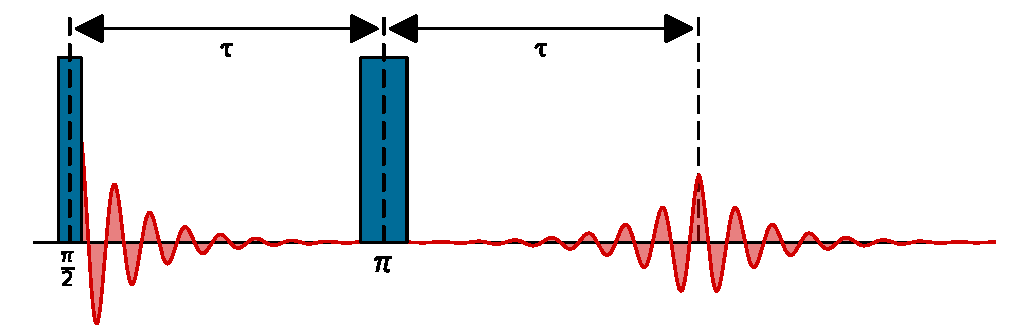
\includegraphics[width=0.9\tw]{figures/relaxometry/SingleEchoT2.pdf}
\caption{The simplest T$_2$ pulse sequence - a single pulse is applied and the signal at 2$\tau$ (at the echo) is measured as a function of $\tau$.}
\label{fig:SpinEchoSequence}
\end{figure}


The observed transverse relaxation constant $T_{2}^*$ is affected by both the dynamic inhomogeneities induced by spin-spin interactions and by static inhomogeneities in the bias offset field. Since the static inhomogeneities are a product of the system and not of the sample, $T_{2}^*$ is not generally a useful measure, except for when characterizing NMR measurement systems. However, the asymmetries between static and dynamic inhomogeneities allows $\mathrm{T}_{2}$ to be measured, even in the presence of inhomogeneous broadening, using a spin-echo pulse sequence (see Fig \ref{fig:SpinEchoSequence}). When a $\pi_{x}$ pulse is applied to $N$ spins initially along $I_{x}$ after time $\tau$, the $\vec{y}$ and $\vec{z}$ components are inverted, effectively applying mirror reflections about $\vec{x}$. Assuming each spin is precessing in its own local field $B_{zj}$ at its own frequency $\omega_{j}$, the density matrix after time $\tau$ is:

\begin{equation}
\label{eqn:InhomogeneouslyBroadenedSpinDensity}
\rho(\tau) = \sum_{j}\cos\left(\omega_{j}\tau\right)I_{x} - \sin\left(\omega_{j}\tau\right)I_{y}.
\end{equation}

The degree of spread in $\omega_{j}$ will determine the coherence of the spin-evolution, and so if $\omega_{j}$ has a wide spread, there will be no signal after a short $\tau$. After applying a $\pi_{x}$ pulse, the density matrix is:

\begin{equation}
\label{eqn:InhomogeneouslyBroadednedAfterPulse}
\rho(\tau+t_{p}) = \sum_{j}\cos\left(\omega_j\tau\right)I_{x} + \sin\left(\omega_{j}\tau\right)I_{y}
\end{equation}

Assuming that the set $\{\omega_{j}\}$ does not change after the pulse, the density matrix after a second period of evolution of time $\tau$ serves to return the spins to their original state:

\begin{align}
 \rho(2\tau+t_{p}) & =  \sum_{j}\cos\left(\omega_{j}\tau\right)\left[\cos\left(\omega_{j}\tau\right)I_{x} - \sin\left(\omega_{j}\tau\right)I_{y}\right] + \sin\left(\omega_{j}\tau\right)\left[\cos\left(\omega\tau\right)I_{y} \right] & \nonumber \\
 & =  \sum_{j}\left[\cos^{2}\left(\omega_{j}\tau\right) + \sin^{2}\left(\omega_{j}\tau\right)\right]I_{x} + \left[\cos\left(\omega_{j}\tau\right)\sin\left(\omega_{j}\tau\right) - \cos\left(\omega_{j}\tau\right)\right]I_{y} & \nonumber \\
 & =  \sum_{j}I_{x} = NI_{x}. &
\label{eqn:SpinRefocusAfter2Tau}
\end{align}

Because of the transient nature of the spin-spin interactions, the dynamic field inhomogeneities are not reversible, as the local field experienced by each spin changes before and after the pulse. Calling $\tilde{\omega}_{j}$ the frequency of spin evolution for spin $j$, the density matrix after $2\tau$ is given not by Eqn. \ref{eqn:SpinRefocusAfter2Tau}, but by Eqn. \ref{eqn:SpinImperfectRefocusing}:

\begin{equation}
\rho(2\tau + t_{p}) = \sum_{j}\cos\left[\left(\omega_{j}-\tilde{\omega}_{j})\tau\right)\right]I_{x} + \sin\left[\left(\omega_{j}-\tilde{\omega}_{j})\tau\right)\right]I_{y}
\label{eqn:SpinImperfectRefocusing}
\end{equation}

And since this is linear in $\omega_{j} - \tilde{\omega_{j}}$, even in the presence of transient effects, all static inhomogeneities cancel out, leaving \textit{only} the dyanmic effects, allowing for measurement of $\mathrm{T}_{2}$ rather than $T_{2}^*$. The simplest $\mathrm{T}_{2}$ detection pulse sequence (in an indirect dimension), then, is a single-echo T$_2$ measurement, as seen in Fig. \ref{fig:SpinEchoSequence}.\citep{Hahn1950}.

\subsection{CPMG Echo Train Pulse Sequence}
\label{Section:Relaxometry-T2-CPMGPulseSequence}
One problem with the single echo pulse sequence used in Sec. \ref{Section:Relaxometry-T2} is that not all irreversible effects depend only on the sample - this happens most commonly when spins are moving with respect to a static inhomogeneity, and as a result there is some asymmetry between the phase accrued before and after the $\pi$ pulse. Most of these effects can be alleviated using the Carr-Purcell-Meiboom-Gill (CPMG) sequence, which consists of a train of $\pi$ pulses spaced at $(2n-1)\tau$ (for $n \in [1, N]$), rather than a single pulse. This serves to refocus the pulses frequently, and prevents much phase from accruing between echoes.\citep{carr-purcell-1954,Meiboom1958}

\begin{figure}[ht!]
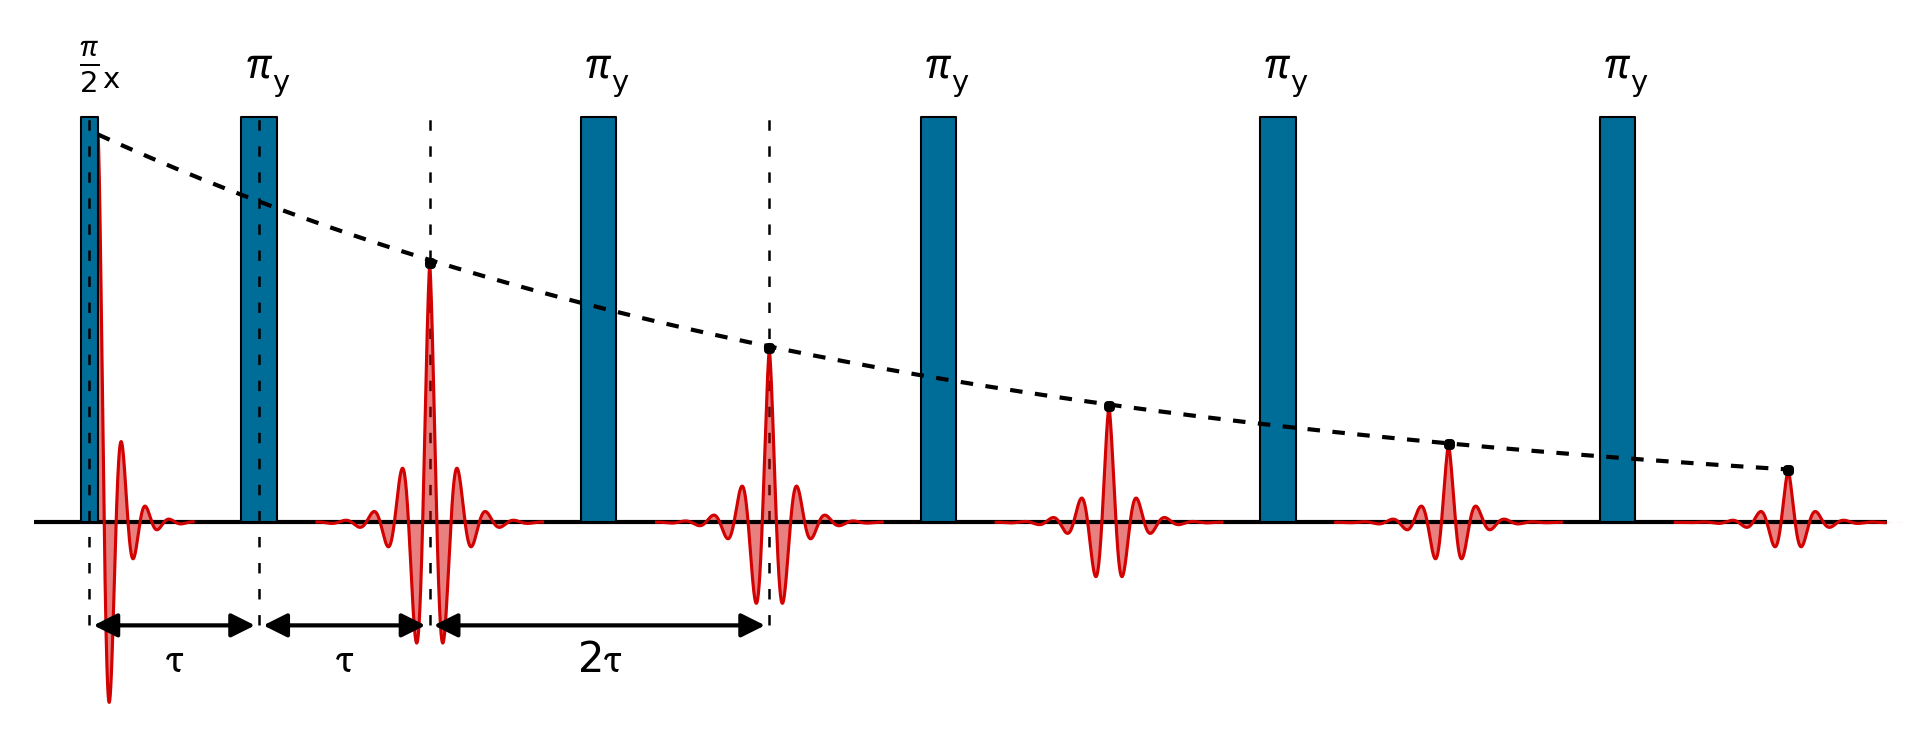
\includegraphics[width=\tw]{figures/relaxometry/cpmg_sequence_demo.png}
\caption{The CPMG sequence is used for making T$_{2}$ measurements.}
\label{fig:CPMGSequence}
\end{figure}

In addition to the moment nulling effects described in Sec. \ref{relaxometry.t2.cpmg.nulling}, the CPMG pulse sequence allows for spins to be refocused before large phase differences accrue. If a sufficiently short $\tau$ is chosen such that the phase accrued over a $2\tau$ period is well-approximated by a linear function (i.e. if the phase is locally linear over the interval $2\tau$), most of the inhomogeneities will refocus under the CPMG pulse, as seen in Fig. \ref{fig:CPMGRefocus}. 

\begin{figure}
\centering
\begin{subfigure}[h]{0.45\tw}
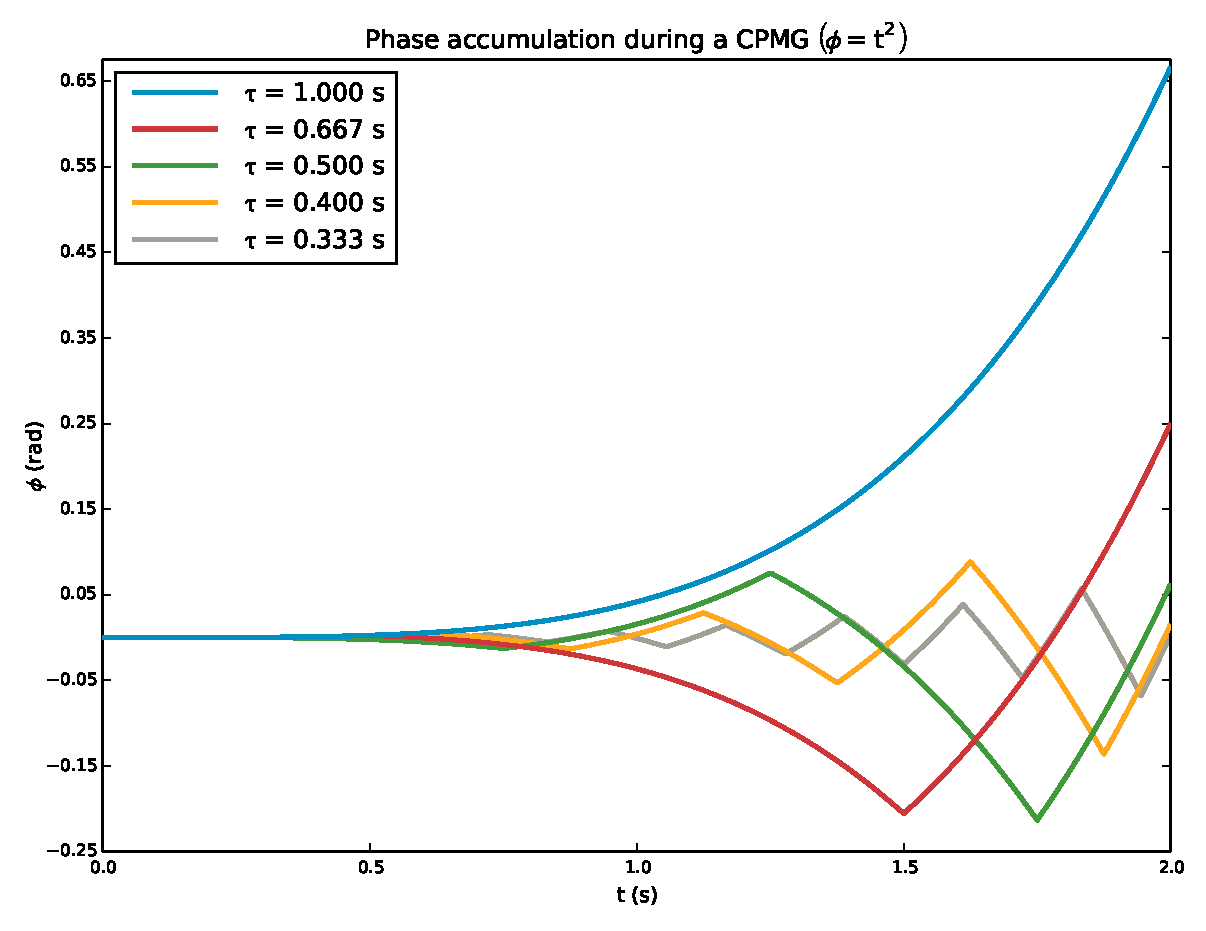
\includegraphics[width=\tw]{figures/relaxometry/PhaseAccumulationt.eps}
\caption{}
\label{sfig:PhaseAccumulationt}
\end{subfigure}
\begin{subfigure}[h]{0.45\tw}
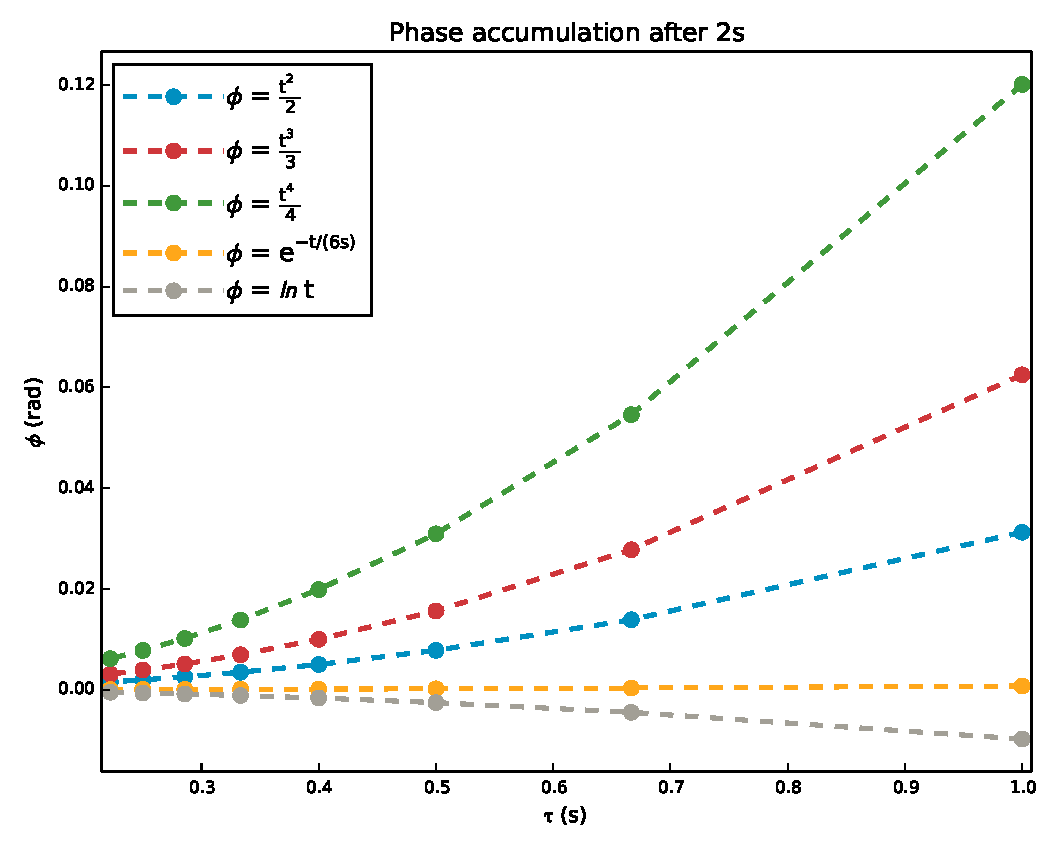
\includegraphics[width=\tw]{figures/relaxometry/PhaseAccumulationTaus.eps}
\caption{}
\label{sfig:PhaseAccumulationTaus}
\end{subfigure}

\caption{The affect of a CPMG sequence on phase accumulation for several non-linear functions of $t$. (\subref{sfig:PhaseAccumulationt}) Although $\phi = e^{-Rt}$ is a non-linear function of $t$, for $\tau \ll R$, the change in the function is small enough that very little phase accumulates. (\subref{sfig:PhaseAccumulationTaus}) The phase accumulation after $N\tau = $\unit[2]{s} as a function of $\tau$ for gradients characterized by several non-linear functions - the degree of phase accumulation is essentially related to the linearity of the function over a given $2\tau$ interval.}
\label{fig:CPMGRefocus}
\end{figure}

There are two ways to use this to more accurately measure T$_{2}$ - in one case, the single-echo sequence is modified to have a large number of pulses of duration $\tau$, and $\tau$ is varied over the course of the experiment, and in the other, the signal at each echo (or some subset of echoes) is measured over $N$ measurements with a constant $\tau$. While the first method is in a sense an improvement over the single-pulse case, there are still many non-linear effects introduced by this method - the effects from convection and diffusion scale as $\tau^2$, and in a constant-$N$ approach, the fraction of time the spins spend in the pulse field is also changing as a function of $\tau$. In a constant-$\tau$ approach, even if practical constraints prevent a sufficiently short $\tau$ to fully eliminate these effects they are at least made significantly more linear, reducing their effects on the signal.   

\subsubsection{Moment Nulling}
\label{relaxometry.t2.cpmg.nulling}
One problem that arises is that the sample is flowing in some way - either due to convection effects, actual fluid flow or sample jostling. In our magnetometry experiments, convection effects and stirring due to sample impact were serious concerns - both causing some mass nuclear movement in the presence of some potential real gradients. For $\tau$ sufficiently short that the spins can be thought of as moving in a linear gradient, we can model the phase accrual after $\tau$ as:\cite{carr-purcell-1954}

\begin{equation}
\phi_{j} = \int_{\tau_{1}}^{\tau_{2}}\left[\omega_{j} + \sum_{m=1}\left(m+1\right)\left(\alpha_{j}^{(m)}t^{m}\right)\right]\mathrm{d}t
\label{eqn:PhaseAccrualMovementTauInt}
\end{equation}

Where $\alpha_{j}^{(m)}$ are a set of coefficients representing phase accrual due to the $m^{th}$ derivative of the position as a function of time, i.e. $\alpha_{j}^{(1)}$ relates to the phase contributed by the velocity, $\tfrac{\partial x}{\partial t}$, and $\alpha_{j}^{(2)}$ represents the phase contributed by the acceleration, etc.\footnote{I have arbitrarily defined the set $\alpha_{j}^{(m)}$ such that the integer factor is included after integration, which is why the sum is defined with each term multiplied by $m+1$.} This evaluates on the interval $[\tau_{1}, \tau_{2}]$ as

\begin{equation}
\phi_{j} = \omega_{j}\tau + \sum_{m=0}\alpha^{(m)}\left(\tau_{2}^{(m)}-\tau_{1}^{(m)}\right).
\label{eqn:PhaseAccrualMovementTauEval}
\end{equation}

For a system limited to only 1st order (velocity) effects, the phase for spin $j$ after $\tau$ is $\phi_{j} = \omega_{j}\tau + \alpha_{j}^{(1)}\tau^2$. Applying a $\pi_{x}$ pulse, the mirror reflection inverts the phase, so $\phi'_{j} = -\omega_{j}\tau - \alpha_{j}^{(1)}\tau^2$. After a second period of evolution (between time $\tau$ and $2\tau$), the spins pick up an additional phase $\omega_{j}\tau + \alpha_{j}^{(1)}\left[(2\tau)^2-\tau^2\right] = \omega_{j}\tau + 3\alpha_{j}^{(1)}\tau^2$. Which gives a total phase of $\omega_{j}\tau + 3\alpha_{j}^{(1)}\tau^2 - \omega_{j}\tau - \alpha_{j}^{(1)}\tau^2 = 2\alpha_{j}^{(1)}\tau^{2}$ - as expected, the asymmetry due to the motion of the spins remains, even when the static inhomogeneities represented by $\omega_{j}$ are canceled out. However, if another $\pi$ pulse is applied at $3\tau$, the first order term cancels out at the second echo:

\begin{align}
\phi & = 2\alpha_{j}\tau^2 \xrightarrow{2\tau\hspace*{1cm}3\tau} \omega_{j}\tau + 7\alpha_{j}\tau^2 \xrightarrow{\hspace*{1.5mm}\pi_{x}\hspace*{1.5mm}} -\omega_{j}\tau - 7\alpha_{j}\tau^2 & \nonumber \\ 
 & = \xrightarrow{3\tau\hspace*{1cm}4\tau} \omega_{j}\tau - \omega_{j}\tau -7\alpha_{j}\tau^2 + 7\alpha_{j}\tau^2 = 0. &
\label{eqn:PhaseCancellation4tau}
\end{align} 

And when the spins have completely refocused, the same exact analysis applies as if the spins are at $\tau = 0$ at the second echo, and so it is clear that the zeroth order (static) inhomogeneities refocus on each echo, while the second order inhomogeneities refocus every other echo. The higher-order components, however, do not naturally refocus using a simple CPMG pulse. At the $n^{th}$ echo, the phase accrued from the 2$^{\mathrm{nd}}$ order effect ($\phi_{n}^{(2)}$) is given by the sum

\begin{align}
\frac{\phi^{(2)}}{\alpha_{j}^{(2)}\tau^3} & = \left(-1\right)^{n}\sum_{m=1}^{n}(-1)^{m}\left[\left(2m\right)^3 - 2\left(2m-1\right)^3 + \left(2m-2\right)^3\right] & \nonumber \\
&  = (-1)^{n}\sum_{m}^{n}\left(-1\right)^{m}\left(12m-6\right) = 6n. & \\
\label{eqn:AccelerationEffectSum}
\end{align} 

From Eqn. \ref{eqn:AccelerationEffectSum} it can be seen that the 2$^{\textrm{nd}}$ order effect is reduced from a polynomial effect to a linear effect at each echo. This is simple to deal with, because linear phases cancel out after a single echo - by applying a $\pi$ pulse \textit{during} the 2$^{\textrm{nd}}$ echo sequence (when both the 0$^{\textrm{th}}$ and 1$^{\textrm{st}}$ order effects have been canceled), at $n = 4$, the 0$^{\textrm{th}}$, 1$^{\textrm{st}}$ and 2$^{\textrm{nd}}$ order effects are fully refocused at $8\tau$. If the same method of analysis is applied to the 3$^{\textrm{rd}}$ order effect, it is found that using this pulse sequence results in a linear phase accruing on even echoes - the pulse sequence can be then modified such that the first 4 components cancel after 8 echoes by removing all the $\pi$ pulses from every other echo (at which point the first 3 components are zero anyway, and so are unaffected by whether or not a pulse occurs). Consider the modified pulse sequence

\begin{equation}
\label{eqn:ModifiedCPMGPulseSequence}
(\tau - \pi_{x} - \tau - \varphi(i))_{n};
\end{equation}

in this sequence, $\varphi_{i}$ is the phase applied at the $i^{\mathrm{th}}$ repetition of the sequence. For optimal cancellation, $\varphi_{i}$ is

\begin{equation}
\label{eqn:2adicvaluationpulses}
\varphi_{i} = \pi\left(\frac{1+(-1)^{v_{2}(i)}}{2}\right),
\end{equation}

where $v_{2}(i)$ (sometimes called $ord_{2}(i)$) is the \textit{2-adic valuation} of $i$ - the multiplicity of the number 2 in the prime factors of $i$. Put another way, for $i = 2^{k}j$ where $i, j, k \in \mathbb{Z}$ and $j$ is an odd number, $v_{2}(i) = k$. This can easily be calculated by counting how many times $i > 0$ can be divided by 2 without returning an odd number. Using this pulse sequence, at the $n^{\mathbf{th}}$ echo, all components $m \leq v_{2}(n)$ are 0 (e.g. at $n = 160 = 5\cdot2^{5}$, $\phi^{(0)} = \phi^{(1)} = \phi^{(2)} = \phi^{(3)} = \phi^{(4)} = \phi^{(5)}$).

\subsubsection{Pulse-time fraction}
\label{relaxation.t2.cpmg.pulse.time}
One last concern to address is the fraction of time that spins feel the pulse field. At high field, this is not a significant effect, as pulses are very small compared to the main bias offset field ($B_0$). The situation is different, however, at low field, where the strength of the pulses is the same order of magnitude as (or larger than) the bias field. This can may cause significant shifts in the measurement of T$_2$ if care is not taken. Because the relaxation operations commute with one another (i.e. $M_{0}e^{-\sfrac{\left(t^{(2)}-t^{(1)}\right)}{\mathrm{T}_{2}^{(1)}}}e^{-\sfrac{\left(t^{(1)}-t^{(0)}\right)}{\mathrm{T}_{2}^{(0)}}} =  M_{0}e^{-\sfrac{\left(t^{(1)}-t^{(0)}\right)}{\mathrm{T}_{2}^{(0)}}}e^{-\sfrac{\left(t^{(2)}-t^{(1)}\right)}{\mathrm{T}_{2}^{(1)}}}$), the overall relaxation constant $\overline{\mathrm{R}}_{2} = \sfrac{1}{\overline{\mathrm{T}}_{2}}$ can be expressed as the integral over the relaxation constants during the period in question - which is the continuous-form equivalent of a time-weighted average of the relaxation times:

\begin{gather}
\label{eqn:VaryingR1}
e^{-\overline{\mathrm{R}}_{2}t} = \prod_{i}e^{\mathrm{R}_{2,i}\Delta t_{i}} = e^{-\sum_{i}\Delta t_{i} \mathrm{R}_{2,i}} \xrightarrow{\hspace*{5mm}}\lim_{n\to\infty}e^{\sum_{i}\Delta t_{i}\mathrm{R}_{2,i}} = e^{\int_{0}^{t}\mathrm{R}_{2}(t)\mathrm{d}t} \\
\overline{\mathrm{R}}_{2}  =  \int_{0}^{t}\mathrm{R}_{1}(t)\mathrm{d}t.
\end{gather}

Taking the greatest difference we've observed in water T$_2$ as a ``worst case'' estimate of the effect, we will assume that we're interested in measuring the zero field T$_{2}$ (T$_{2,zf}$), and pulses are applied at \unit[27]{mG} where $t_{p} \approx $ \unit[27]{ms}\footnote{This is actually a quite low pulse field. Standard pulses are generally on the order of \unit[100]{$\mu$s}, and ``low intensity'' pulses are on the order of \unit[1]{ms}}. At $\approx$ \unit[37]{\degsym C}, T$_{2,zf} \approx$ \unit[2.88]{s} and T$_{2,27\mathrm{mG}} \approx $ \unit[2.39]{s}. Assuming the relaxation is only changing in response to the different field at the pulse, then:

\begin{equation}
\label{eqn:AvgRelaxationRate}
\overline{\mathrm{R}}_{2} = \frac{t_{p}\mathrm{T}_{2,zf} + t_{m}\mathrm{T}_{2,27\mathrm{mG}}}{\mathrm{T}_{2,27\mathrm{mG}}}\mathrm{T}_{2,zf}\left(t_{p} + t_{m}\right)
\end{equation}

 Where $t_{m}$ is the time between pulses. Given the length of $t_{p}$, the most probable value for $t_{m}$ is $\approx$ \unit[73]{ms} (such that $t_{p} + t_{m} =$ \unit[100]{ms}), so $\overline{\mathrm{R}}_{2} = $\unit[0.362]{s$^{-1}$} and $\overline{\mathrm{T}}_{2} = $ \unit[2.52]{s} - an error of $\approx$ 5\%. In a typical case, a T$_2$ measurement would be made at \unit[0.5]{G} using pulses either at \unit[114]{mG} ($t_{\pi}$ = \unit[1.03]{ms}) or at \unit[1.1]{G} ($t_{\pi} =$ \unit[107]{$\mu$s}). Under the same conditions as in the earlier analysis, at \unit[0.5]{G}, T$_2 \approx$ \unit[2.88]{s}. At \unit[114]{mG}, T$_2 \approx$ \unit[2.59]{s}, and for typical value $\tau $ = \unit[20]{ms}, the measured $\overline{\mathrm{T}}_{2}$ would be \unit[2.86]{s} a bias of $\approx$ 0.5\%. At \unit[1.1]{G}, T$_2 \approx$ \unit[2.91]{s}, and for typical value $\tau $ = \unit[5]{ms}, the measured $\overline{\mathrm{T}}_{2}$ would be \unit[2.885]{s}, an error of $\approx$ 0.2\%. Although the difference in T$_2$ can be arranged to be an insignificant source of error, it is still necessary to consider during data processing, as often when applying long CPMG trains the fraction of time spent pulsing is a considerable fraction of the pulse sequence.  Additionally, it is worth noting that these calculations make the assumption that the spins are relaxing due to the homogeneously-broadened T$_2$, not the inhomogeneously-broadened coil T$_2^*$ - which may be \textit{much} shorter. This, however, can be alleviated by alternating the direction of the $\pi$ pulses between $\vec{x}$ and $\vec{y}$, which act to mutually correct their static inhomogeneities, for reasons detailed in the context of pulse error correction in Sec, \ref{nmr.signal.magnetization.pitrain.variations}.
  
\section{Diffusometry Measurements - Methods}
\label{Section:Relaxometry-Diffusion}
While it may necessitate error correcting pulse sequences, the fact that spins moving through static inhomogeneities are imperfectly canceled by spin echo pulse sequences is quite useful for measuring fluid flow (as in many velocity and acceleration imaging applications) and diffusion. Like T$_1$ and T$_2$, the diffusion properties of spins is an inherent property of a system, and can be used as a proxy for many important measurements like temperature, viscosity, fat content in dairy products, etc.\cite{kopf-biophys-1996,guthausen-jaocs-2004}

\subsection{Pulse Sequences}
\label{Section:Relaxometry-Diffusion-PulseSequence}
\begin{figure}[ht!]
\centering
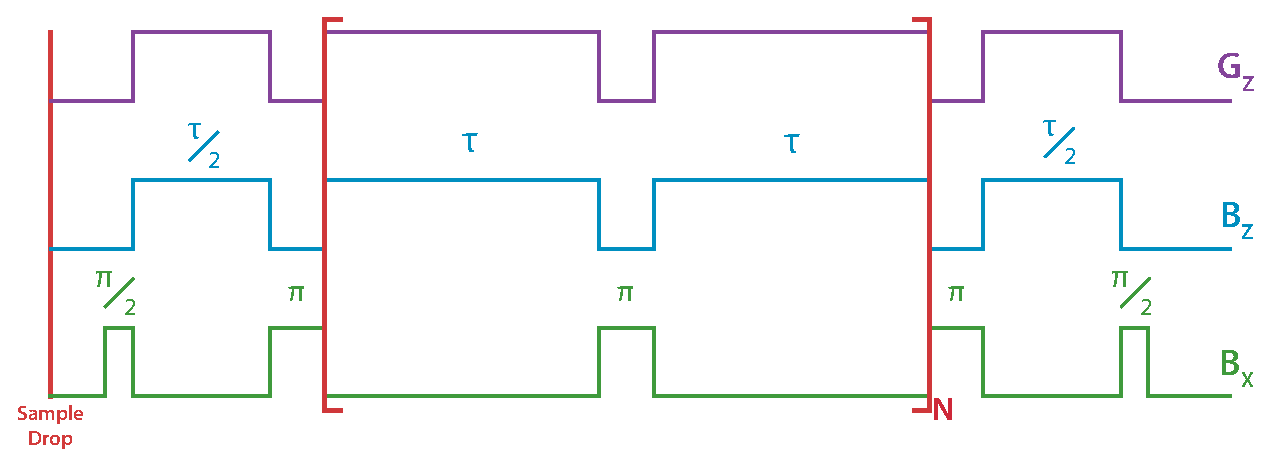
\includegraphics[width=0.9\tw]{figures/relaxometry/DiffusionPulseSequence.eps}
\caption{The most basic diffusion pulse sequence is a CPMG pulse sequence in the presence of an applied gradient $G_{z}$.}
\label{fig:DiffPulseSequence}
\end{figure}

Unlike in the examples of fluid flow and convection, wherein a persistent direction of flow causes phase to grow (on most time-scales) fairly linearly - or at least by a function which is well-fit to a low-order polynomial - diffusing spins are effectively executing a random walk, and the position of a given diffusing spin is increasingly uncorrelated with its starting position. The non-refocused phase accumulation for spins diffusing in a linear gradient of strength $G$ after an echo ($t = \tau$) comes from the root-mean-square distribution of the spins\footnote{$\sqrt{\left\langle x^2\right\rangle} = \sqrt{\left\langle y^2\right\rangle} = \sqrt{\left\langle z^2\right\rangle} = \sqrt{2Dt}$}, and is given in Eqn. \ref{eqn:DiffusionPhase}:

\begin{equation}
\label{eqn:DiffusionPhase}
\phi_D = (\gamma G D)^2\frac{t^3}{3}
\end{equation}

Thus the signal after time $\tau$ is:

\begin{equation}
\label{eqn:Diffusionsignal}
M(t) = M_{0}e^{-\sfrac{t}{T_{2}}}e^{-\sfrac{\left(\gamma G\right)^2D\tau^3}{3}}
\end{equation}

Assuming that the different periods of evolution commute (which should be true for the assumed motion in a linear $\sfrac{\partial B_{z}}{d z}$ gradient), repeated applications of the spin echo sequence add linearly, and so after a CPMG pulse train of length $N$, the signal is:\cite{f-exp-pulse-nmr}

\begin{align}
\label{eqn:DiffusionSignalCPMGt}
M(t) & = M_{0}e^{-\sfrac{t}{\mathrm{T}_{2}}}e^{-\sfrac{N\left(\gamma G\right)^2D\tau^3}{3}} \\
& = M_{0}e^{-\sfrac{t}{\mathrm{T}_{2}}}e^{-\sfrac{\left(\gamma G \tau\right)^2Dt}{3}}
\label{eqn:DiffusionSignalCPMGtau}
\end{align} 

Where Eqn. \ref{eqn:DiffusionSignalCPMGtau} is found by substituting $t = N\tau$ into Eqn. \ref{eqn:DiffusionSignalCPMGt}. When making $\mathrm{T}_{2}$ measurements, it is necessary to choose a $\tau$ sufficiently small that diffusion effects are minor, whereas when measuring diffusion, it's necessary to make measurements which minimize the signal asymmetries due to anything but diffusion. In Eqn. \ref{eqn:DiffusionSignalCPMGtau} the signal is proportional to three different control variables - $N$, $\tau$ and $G$. Varying either $G$ or $\tau$ gives a one-sided Gaussian decay ($e^{-x^2}$), while varying $N$ gives a simple exponential decay ($e^{-x}$), however varying $N$ or $\tau$ also necessarily varies $t$, and the exponential in Eqn. \ref{eqn:DiffusionSignalCPMGtau} can be expressed as $-t\left[\sfrac{1}{\mathrm{T}_{2}} + \sfrac{\left(\gamma G\tau\right)^{2}D}{3}\right]$, and so the output will not be a pure function of diffusion. That said, it may be acceptable to vary $t$ when $\sfrac{\left(\gamma G \tau\right)^{2}D}{3}\gg\sfrac{1}{\mathrm{T}_{2}}$. In general, though, the greatest symmetry is achieved by acquiring signal while varying $G_{z}$, as the pulse sequence is identical save for the gradient strength - which affects only moving components of the spin echo sequence, and with the right choice of pulse sequence, effects like convection or residual angular momentum in the sample can be easily nulled.

One major concern that can be limiting is the choice of $N$ and $\tau$ - which determine the speed of the Gaussian decay, as well as the total time $t$ of each run. Ideally $G_{z}$ will be swept at least through the linear region of the curve, and preferably until the signal fully decays. For example, to sweep through the curve from 0 decay due to diffusion up to at least 95\% decay due to diffusion, $N$, $\tau$ and $G_{z}$ should be chosen such that $\sfrac{\left(\gamma G_{max}\tau\right)^{2}Dt}{3} \geq -\mathrm{ln}(0.95) \approx -0.0513$. Generally $G_{max}$ will be the limiting factor - either the fundamental limits of the pulsing circuit, the coil or the shields will prevent the gradient from increasing too much and remaining linear. Holding $\gamma G_{max}$ constant, the equation can then be expressed as:

\begin{equation}
\label{eqn:OptimalNTaus}
N\tau^3 \geq -\frac{3\mathrm{ln}(0.05)}{\gamma^{2}G_{max}^{2}D}
\end{equation}

Unfortunately, with this approach, a full $\mathrm{T}_{2}$ curve is not measured, and so all the signal earlier in the sequence is eliminated. As a result, $t=N\tau$ should be minimized with respect to Eqn. \ref{eqn:OptimalNTaus}, and $N$ should be constrained to be an even multiple of 4 or, if possible, 8, as this allows for nulling of the first few orders of motion terms. Minimizing $N\tau$ for a given value of $N\tau^3$ is clearly done by using the smallest possible value of $N$, as the minimized function grows linearly in $N$, but as the cube root of $\tau^3$, and so the solution is then to choose $N$ = 4 or 8 (depending on the strength of the higher-order corrections), so $\tau$ is given by:

\begin{equation}
\tau \geq \sqrt[3]{\frac{-3\mathrm{ln}(0.05)}{N\gamma^2G_{max}^{2}D}}
\end{equation}

For a typical value of $G_{max} = $\unitfrac[0.4]{G}{cm}, the self-diffusion coefficient for water at T=\unit[300]{K} is $D =$\unitfrac[2.35$\cdot$10$^{-5}$]{cm$^2$}{s},\cite{Wang1965} $\tau_{4} \approx$ \unit[94]{ms} and $\tau_{8} \approx $ \unit[75]{ms} with $t_{4} =$ \unit[376.5]{ms} and $t_{8} =$ \unit[597.5]{ms}. For T$_{2} \approx$ \unit[2.4]{s}, this represents a loss of 15\% and 22\% of signal, respectively. Ideally, the gradient strength would be greatly increased, allowing for much shorter values of $\tau$ - this is mainly problematic in some shielded magnetometry applications due to the fringe field from the gradient, which can serve to magnetize the innermost layer of shielding.

% \subsection{Concomitant Gradients}
% \label{relaxometry.diff.concomitant}
% The analysis in previous sections have relied on our ability to create a pure $\sfrac{\partial B_{z}}{\partial z}$ gradient, but this is something that is not possible according to Maxwell's equations. Specifically, Gauss's law for magnetism:

% \begin{equation}
% \label{eqn:GaussLawMagnetism}
% \nabla\cdot\mathbf{B} = \left(\frac{\partial B_{x}}{d x}\right) + \left(\frac{\partial B_{y}}{\partial y}\right) + \left(\frac{\partial B_{z}}{\partial z}\right) = 0 
% \end{equation}

% Eqn. \ref{eqn:GaussLawMagnetism} requires that for a given gradient $G_{z}$, there should be concomitant gradients $G_{x} + G_{y} = -G_{z}$. This is not normally a problem at high magnetic field, because the transverse components of the field are truncated by the presence of a large bias magnetic field - for the same reason that off-resonance pulsing has no effect on the spins, the average effect of relatively small transverse fields on rapidly precessing spins averages to zero. At low field, however, this truncating field may not be relied on to truncate the effects of the concomitant gradients, and some effort needs to be made to deal with these. Generally, a small field ($\approx$ \unit[0.5]{G}) is applied during the measurements, both to simulate earth's field detection and to add in a small truncating field - since fairly small gradients are used to avoid shield magnetization, this is often sufficient to truncate the transverse components - however, increased gradient strength is very valuable for increasing signal and resolution, and so weak gradients are a non-ideal solution to the problem of concomitant gradients.

% A more palatable solution is the use of a multi-phase decoupling sequence in place of the standard CPMG pulse sequence, similar to those used in Secs. \needcite{Figure out all the places I use multi-phase pi trains}. While such a sequence does not remove contributions from diffusion along transverse axes - which can complicate matters somewhat - it is certainly possible to remove the decoherence due to inhomogeneous broadening by alternating the phase of the CPMG pulses between $\vec{x}$ and $\vec{y}$. The phase of the pulses makes no difference to the outcome of the $\vec{z}$ magnetization, but a pulse along $\vec{x}$ causes an echo along both $\vec{y}$ and $\vec{z}$, while a $\pi$ pulse along $\vec{y}$ causes an echo along $\vec{x}$ and $\vec{z}$. Using this, we can replace each single echo with a 4-echo sequence, shown in Fig. \ref{fig:DiffusionCPMGConcomtant}\needfig{Figure demonstrating the multiphase CPMG's effect on concomitant gradients - 4 pulses.}

% \begin{figure}[ht!]
% \caption{When accounting for concomitant echoes, each pulse is replaced by a 4-pulse sequence.}
% \label{fig:DiffusionCPMGConcomtant}
% \end{figure}

% With the phase configuration shown, the components along $\vec{z}$ echo at $n\tau$, while the component along $\vec{x}$ echoes at $\tau$ and $4\tau$, and the component along $\vec{y}$ echoes at $3\tau$ and $4\tau$. If the same sequence is run again (or run again with the sequence inverted - it makes no difference), each component will have echoed an even number of times, $\vec{z}$ landing on its 8$^{\mathrm{th}}$ echo at spacing $\tau$, and $\vec{x}$ and $\vec{y}$ with 2 echoes of duration $\tau$ and $3\tau$. At this point, the static phase and 1$^{\mathrm{st}}$ order (velocity) terms have canceled in 8 pulses. Unfortunately, canceling the next higher order terms requires repeating this sequence 4 more times - with alternating $\vec{x}$ and $\vec{y}$ pulses at $4n\tau$ - but hopefully if the gradients are weak enough that applying 64 pulses is problematic, then the higher-order terms will not make a significant contribution to the signal decay.

% Another option which significantly reduces the number of pulses required is by removing the $\pi$ pulses entirely and inverting the applied $G_{z}$ gradients. Because the gradient coils are the source of both the main gradient and the concomitant gradient, inverting the current through the gradient inverts all three components of the spin magnetization, not just two (as is the case in pulses). This allows each time period $\tau$ to be treated as if the right pulses are being applied along both $\vec{x}$ and $\vec{y}$ at the same time. 


\section{Measurements of Hydrocarbons and Water}
\label{relaxometry.hydrocarbons}
Relaxometry and diffusometry are used extensively in portable and \textit{ex-situ} NMR applications, as these techniques can be applied even in grossly inhomogeneous fields for characterization of bulk heterogeneous materials.\cite{hurlimann-jmr-2000,song-nmr-chemical-engineering-2006} These techniques for the basis for nearly all NMR methods for oil well logging, where the ``sample'' is fluid in rock formations surrounding a well bore. As the Earth's field is generally homogeneous over very large regions, Earth's field detection has the potential to vastly increase the effective sample volume of NMR measurements performed without a bias offset field.

To this end, we performed a number of experiments using an atomic magnetometer to measure relaxation and diffusion in samples of pure hydrocarbons and water at Earth's field as an initial proof of concept that atomic magnetometers have the chemical sensitivity required to quantitatively and qualitatively distinguish between hydrocarbons and water. The experiments are described in detail in Sections \ref{Section:Relaxometry-T1}, \ref{Section:Relaxometry-T2} and \ref{Section:Relaxometry-Diffusion} - all are performed in an indirect dimension at \unit[0.5]{G}. Although all measurements were made at zero field, \slrel{} and \ssrel{} measurements are sensitive to the magnetic field and so during the experimental evolution \unit[0.5]{G} was chosen to best emulate the strength of the Earth's ambient magnetic field; diffusion is not sensitive to magnetic field strength,\footnote{At least not in solvents. It is conceivable that magnetic field strength could have an effect on diffusion in ferrofluids or other magnetic liquids.} but the degree to which concomitant gradients are truncated by the presence of a bias offset field will indeed be sensitive to the bias offset field.

\subsection{Pure solvents}
\label{relaxometry.hydrocarbons.pure}
The first test performed was to measure relaxation and diffusion in an array of pure solvents to show that the technique has sufficient chemical resolution to distinguish between an array of substances. Measurements were performed on a number of solvents including water, methanol, ethanol and an array of alkanes of increasing chain length. Because \slrel{} and \ssrel{} are functions of both temperature and magnetic field and these experiments were performed at both a lower magnetic field (\unit[0.5]{G}) and a higher temperature (\unit[37]{\degsym C}, due to proximity to the cell) than is common, literature values are not generally available for comparison. 

\subsection{Mixtures}
\label{Section:Relaxation-Diffusion-Hydrocarbons-Mixtures}
As our experiments are intended as a proof-of-concept of the utility of magnetometry at Earth's field for the measurement of heterogeneous materials, it was desirable to make measurements of mixtures of hydrocarbons and water. However, the relatively small sensitive radius of our particular magnetometer (see Sec. \ref{Section:NMR-Detectable-Region}), and the fact that the magnetometer is located directly \textit{below} the sample is a problem, as any physical mixture of immiscible liquids will separate into a bilayer, with the denser material on bottom (close to the sensor) and the lighter material on top, leading to a bias in any quantitative analysis. As such, it was necessary to develop a strategy wherein there was either no longitudinal bias in the sample distribution, or a known and characterized bias for which we can compensate. The latter approach is undesirable, as it introduces model error into the quantification.

\subsubsection{Emulsions}
\label{Section:Relaxation-Diffusion-Hydrocarbons-Mixtures-Emulsions}
The first approach we took in addressing the problem of mixture separation was to use some surfactant in an attempt to create stable emulsions of hydrocarbon solvents and water. The most effective emulsifying agent was a small amount of dish soap added to the water, followed by long periods of sonication. A longer period of sonication leads to the creation of smaller bilayer domains, and significantly increased the stability of the emulsion. After an hour or more of sonication, decane-water emulsions stored at room temperature and at rest were, by visual inspection, stable for over a day, and 1-dimensional relaxation measurements made of the samples were both qualitatively and quantitatively accurate. However, the stable lifetime of the emulsion was found to be significantly reduced at the elevated temperature necessitated by close proximity to the magnetometer cell, combined with the physical disruption provided by the rapid pneumatic shuttling of the sample. Because in our system 2-dimensional relaxation measurements were taken over the course of 12-24 hours, this introduced artifacts into the measurement as the sample components slowly separated out over the course of the measurement.

\subsubsection{Physical Separation}
\label{Section:Relaxation-Diffusion-Hydrocarbons-Mixtures-PhysicalSeparation}
Physically separating the layers using a longitudinal barrier can cause some loss of overall signal, as the barrier will take up some of the sample volume, but has several distinct advantages over emulsions. In addition to solving the issue of the stability of the separation, it also preserves the physical properties of the separated components, and so the T$_1$, T$_2$ and diffusion measurements are unlikely to be affected by the domain size of the emulsion or interactions with the surfactant.

Ideally, we would have used specialized NMR tubes with a thin longitudinal barrier to evenly separate the two substances, but the much more practical solution was to use nested tubes, such as those used in high-field susceptibility matching experiments. In our experiments, we used \unit[3.3]{mm} coaxial inserts from Wilmad-Labglass (part number 517-INNER), which was fit into a standard \unit[5]{mm} NMR tube (part number 517-OUTER), and kept in place with a small spacer (part number 517-SPACER). Using a coaxial insert, there is some asymmetry between the inner and outer sample volumes. Assuming a hemispherical bottom with the same radius $r$ as the radius of the cylindrical portion of the tube, the volume of liquid in an NMR tube filled to height $h > r$ is given by:
\begin{equation}
V(h) = \pi{}r^2\left(h-\sfrac{r}{3}\right).
\label{eqn:VolumeAnyTube}
\end{equation}

With a coaxial insert with inner radius $r_{I}$ and glass thickness $t_{I}$ in a larger NMR tube with inner radius $r_{O}$, the volume of the inner NMR tube to height $h$ is thus

\begin{equation}
V_{i}(h) = \pi{}r_{I}^2\left(h-t_{I}-\sfrac{r_{I}}{3}\right),
\label{eqn:VolumeInnerTube}
\end{equation}

and the volume outside the NMR tube is

\begin{equation}
V_{o}(h) = \pi{}h\left[r_{O}^2-\left(r_{I}+t_{I}\right)^2\right] + \frac{\pi}{3}\left[\left(r_{I}+t_{I}\right)^3 - r_{O}^3\right].
\label{eqn:VolumeOuterTube}
\end{equation}

In our experiments, we used \unit[4.97]{mm} NMR tubes with thickness \unit[0.38]{mm}, and coaxial inserts with \unit[3.3]{mm} outer diameter and \unit[0.1]{mm} thickness, so $r_{O}$ = \unit[2.11]{mm}, $r_{I}$ = \unit[1.55]{mm}, $t_{I}$ = \unit[0.1]{mm}. For all practical purposes, all signal comes from the bottom \unit[2]{cm} of the tube. In this configuration, $V_{I}$ = \unit[146]{$\mu$L}, $V_{O}$ = \unit[102]{$\mu$L}, and so 41\% of the fluid is in the outer volume, with the remaining 59\% in the inner volume. The total volume of the first \unit[2]{cm} of the larger NMR tube is \unit[372]{$\mu$L}, so approximately 33\% of signal is lost due to the presence of the coaxial insert.

\subsection{Results}
\label{Section:Relaxation-Diffusion-Hydrocarbons-Results}
\subsubsection{Pure Solvents}
Measurements of these samples were necessarily made at elevated temperatures due to the high temperature environment in the vicinity of the cell. Active cooling with dry nitrogen (see \ref{Section:Pneumatic-Shuttling-Probe-Head-Design}) was used to bring the samples down to $\approx$\unit[37]{\degsym C}. As a proof of concept of the sensitivity of the technique, $\mathrm{T}_{1}$ and $\mathrm{T}_{2}$ were measured for a variety of different solvents at \unit[0.5]{G}. The results are summarized in Table \ref{Table:T1T2DataParams}.

\begin{table}[h]
\centering
\tabulinesep=1.5mm
\begin{tabu} spread 0.85\tw {X[1.5,m,l]X[m,c]X[m,c]X[m,c]} \hline
Compound 	& T$_1$ (s)			& 	T$_2$ (s) 		& D ($\cdot{}10^{-5} cm^2\cdot{}s^{-1}$) \\ \hline
Water 		& 3.27 $\pm $ 0.15 	& 2.08 $\pm$ 0.13 	& 2.6 $\pm$ 0.3  	\\ 
Methanol 	& 2.88 $\pm$ 0.08 	& 2.50 $\pm$ 0.05 	& 3.7 $\pm$ 0.2  	\\ 
Ethanol 	& 2.07 $\pm$ 0.06 	& 2.07 $\pm$ 0.06 	& 2.6 $\pm$ 0.1	 	\\ 
Hexadecane 	& 0.75 $\pm$ 0.03 	& 0.65 $\pm$ 0.02 	& --- 		 	\\ 
Limonene 	& 1.62 $\pm$ 0.04 	& 1.40 $\pm$ 0.10 	& 2.5 $\pm$ 0.2  	\\ 
Heptane 	& 1.91 $\pm$ 0.04 	& 1.70 $\pm$ 0.07 	& 7.0 $\pm$ 0.7	 	\\ 
Octane 		& 1.83 $\pm$ 0.08 	& 1.67 $\pm$ 0.03 	& 4.6 $\pm$ 0.4  	\\
Decane 		& 1.56 $\pm$ 0.07 	& 1.32 $\pm$ 0.08 	& 1.46 $\pm$ 0.07	\\ \hline
\end{tabu}
\caption{Relaxation times and diffusion coefficients of some common solvents measured at \unit[0.5]{G} and approximately \unit[37]{\degsym C}}
\label{Table:T1T2DataParams}
\end{table}

The measurements were limited to water and small-chain alkanes and alcohols because larger molecules tend to have a faster relaxation rate, and the \unit[700]{ms} effective $\mathrm{T}_{1}$ filter imposed by the pneumatic shuttling time places a lower limit on the measurable relaxation times. Despite this, our experiments demonstrate a high degree of chemical sensitivity, with signal-to-noise sufficiently low that it is possible to confidently distinguish between almost any two components based only on their measured $\mathrm{T}_{1}$ and $\mathrm{T}_{2}$ values. All single component data were fit using a least squares curve fit to a single exponential decay. 

Diffusion data are extremely sensitive to temperature, and because the temperature of the sample could not be monitored externally, it is hard to determine the accuracy of these values. These data were gathered on different days, likely using different nitrogen flow conditions and potentially different cell temperatures, and so it is not unlikely that the temperatures at which these data were acquired would be radically different.

\label{Section:Relaxation-Diffusion-Hydrocarbons-Results-Pure-Solvents}
\subsubsection{Mixtures}
\label{Section:Relaxation-Diffusion-Hydrocarbons-Results-Mixtures}
More directly relevant to the problem of heterogeneous material characterization is the ability to (hopefully quantitatively) distinguish components from mixtures of fluids. These experiments were performed using decane and water as a test case, using the coaxial-insert physical separation method described in Sec. \ref{Section:Relaxation-Diffusion-Hydrocarbons-Mixtures-PhysicalSeparation}. 

\begin{figure*}[h!]
\centering
    \begin{subfigure}[t]{0.48\tw}
        \centering
        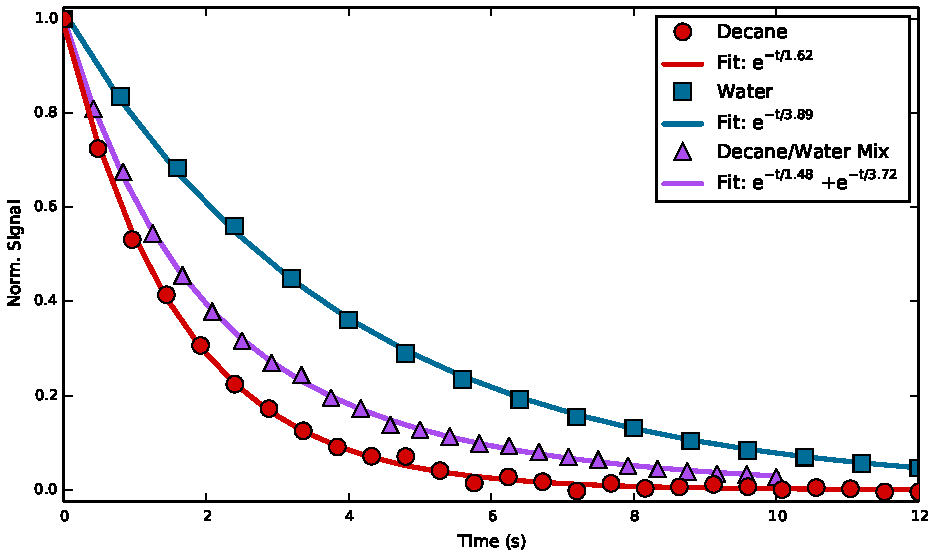
\includegraphics[width=\textwidth]{figures/relaxometry/decane-water-t1.pdf}
        \caption{}
        \label{fig:Decane-Water-T1-Data}
    \end{subfigure}
    \begin{subfigure}[t]{0.48\tw}
        \centering
        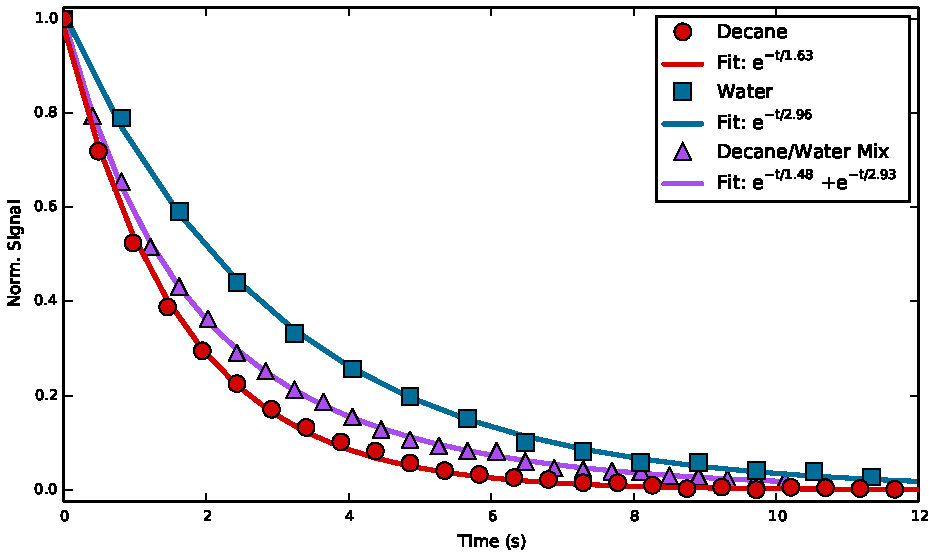
\includegraphics[width=\textwidth]{figures/relaxometry/decane-water-t2.pdf}
        \caption{}
        \label{fig:Decane-Water-T2-Data}
    \end{subfigure}

    \caption{$\mathrm{T}_{1}$ (\ref{fig:Decane-Water-T1-Data}) and $\mathrm{T}_{2}$ (\ref{fig:Decane-Water-T2-Data}) relaxation measurement data.}
    \label{fig:Decane-Water-Relaxation-Data}
\end{figure*}

\begin{figure}[h!]
    \centering
    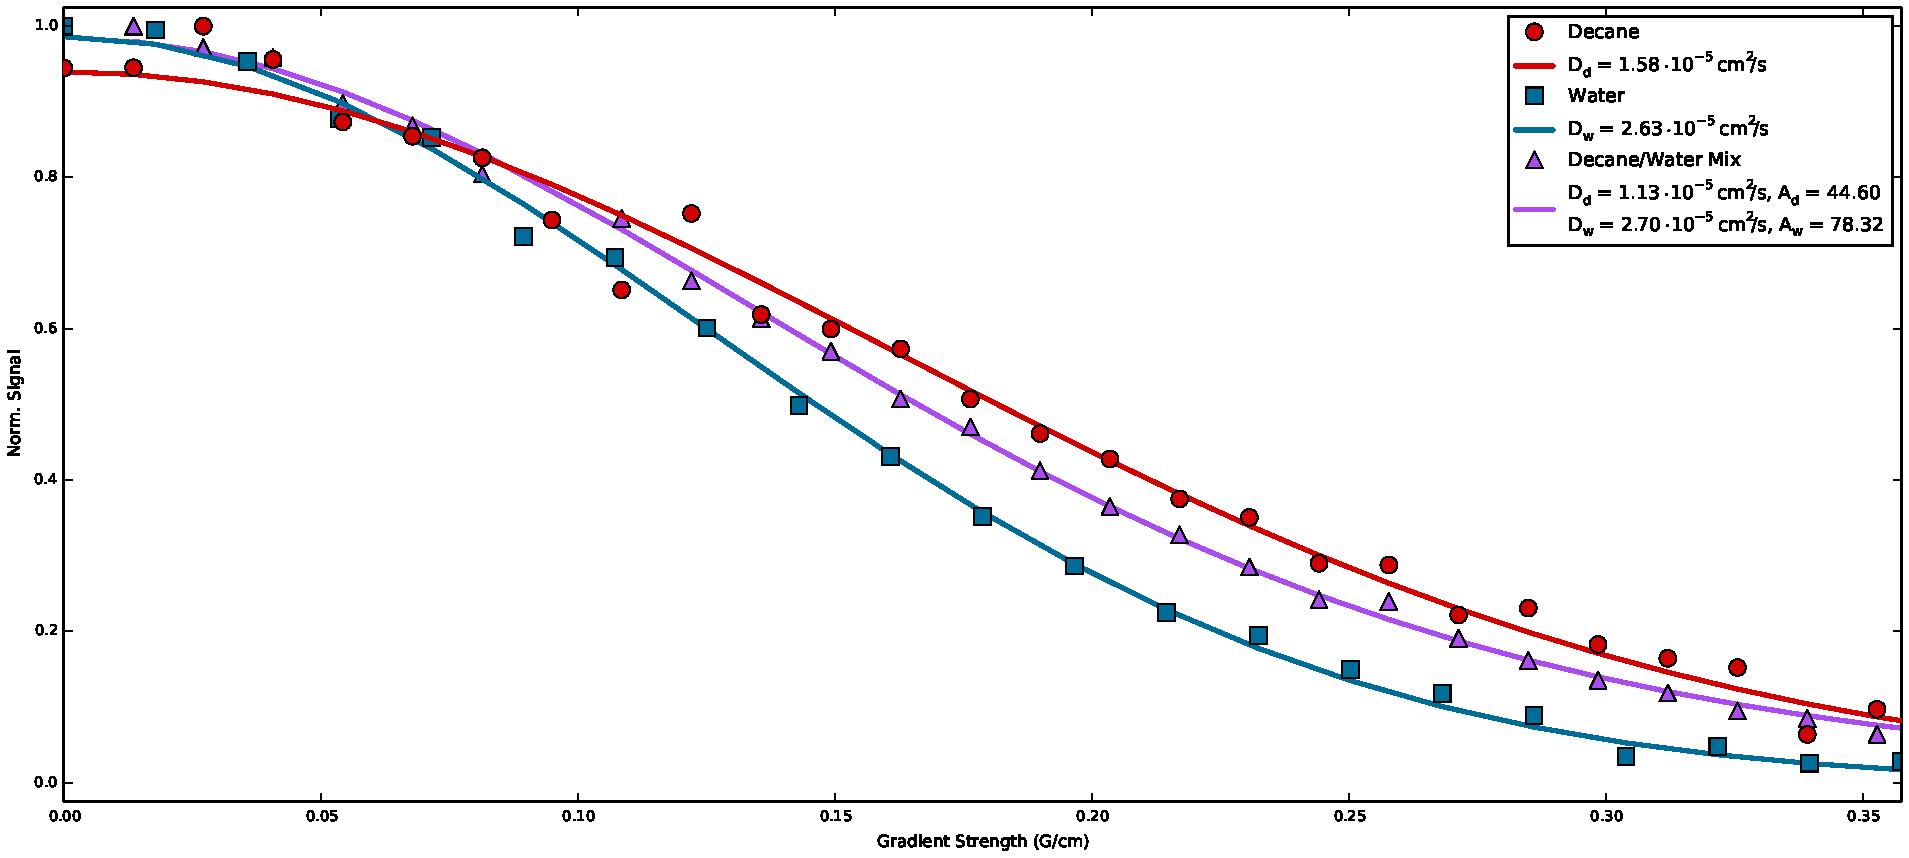
\includegraphics[width=\textwidth]{figures/relaxometry/decane-water-diff.pdf}
    \caption{Diffusion measurements of water, decane and a decane-water mixture.}
    \label{fig:Decane-Water-Diffusion-Data}
\end{figure}

The $\mathrm{T}_{1}$ experiments were performed using the simple shuttle-delay-acquire pulse sequence described in Sec. \ref{Section:Relaxometry-T1-PulseSequence}. As with all the other experiments described in this section, the data were acquired in an indirect dimension, field-cycled to \unit[0.5]{G} to approximate the Earth's ambient magnetic field.

The $\mathrm{T}_{2}$ experiments were performed using the CPMG sequence described in Sec. \ref{Section:Relaxometry-T2-CPMGPulseSequence}, with the time between pulse and echo ($\tau$) set to \unit[5]{ms}, sampled in an indirect dimension at echo numbers $n$ where $n$ was constrained to be an even number to minimize any potential convection or motion effects.

The diffusion experiments were performed using the pulse sequence described in Sec. \ref{Section:Relaxometry-Diffusion-PulseSequence}, with the number of echoes before acquisition, $N$, constrained to be 6 and $\tau$ is set at \unit[75]{ms} and the gradient strength was varied between 

The data from each experiment were fit to a least squares curve fit to the appropriate kernel function --- the results are shown in Figs \ref{fig:Decane-Water-Relaxation-Data} and \ref{fig:Decane-Water-Diffusion-Data}. The relaxation times and diffusion coefficients found in the mixtures can be directly compared to those in the pure solvents to show that this technique is sufficient for separating out the components of hydrocarbon/water mixtures in a qualitative manner. From the amplitudes of the respective signals, we can also extract quantitative information, though it is somewhat less straightforward.

To signal generated from the sample will depend on the prepolarization and shuttling step, which acts as a $\mathrm{T}_{1}$ filter, and differentially affects the different components. For the relaxation experiments, the fraction of signal from a given component, $f_{c,R}$ is calculated from Eqn. \ref{eqn:RelaxationSignalFraction}

\begin{equation}
f_{c,R}  =  \frac{\rho_{H,c}\cdot V_{c}\cdot e^{-t_s/T_{1,c}}}{\sum\limits_{i}\rho_{H,c_{i}}\cdot V_{c_{i}}\cdot{}e^{-t_{s}/T_{1,c_{i}}}},
\label{eqn:RelaxationSignalFraction}
\end{equation}

where $V_{c}$ is the volume of a given component in the set of all components $c_{i}$ and $\rho_{H,C}$ is the hydrogen density. In diffusion experiments, the signal fraction ($f_{D,c}$) also depends on the $\mathrm{T}_{2}$ relaxation occurring during the pulse sequence itself:

\begin{align}
f_{c,D} = \frac{\rho_{H,c}\cdot V_{c}\cdot e^{-t_s/T_{1,c}}e^{-2n\tau/T_{2,c}}}{\sum\limits_{i}\rho_{H,c_{i}}\cdot V_{c_{i}}\cdot{}e^{-t_{s}/T_{1,c_{i}}}e^{-2n\tau/T_{2,c_{i}}}}.
\label{eqn:DiffusionSignalFraction}
\end{align}

These calculations are complicated somewhat by the fact that the $\mathrm{T}_{1}$ relaxation during the shuttling time does not necessarily take place in the fixed \unit[0.5]{G} field induced by the z coil, but rather passes at an unknown speed through a somewhat more complicated field environment generated by, at various times, the prepolarizing magnet, the leading coil, and the $B_z$ coil, making calibration somewhat difficult. At \unit[0.5]{G}, the $\mathrm{T}_{1}$ of water does not seem particularly sensitive to field (see Sec. \ref{relaxometry.dynamics} for more details), and so this does not seem to be a major source of uncertainty.

Applying Eqns. \ref{eqn:VolumeInnerTube} and \ref{eqn:VolumeOuterTube}, we calculate the sample volumes to be $V_{d}$ = \unit[53$\pm$1]{$\mu{}L$} and $V_{w}$ = \unit[59$\pm$1]{$\mu{}L$}. The hydrogen densities for water and decane are $\rho_{H,d}$ = \unit[112.95]{M} and $\rho_{H,w}$ = \unit[110]{M}. Using the measured values of $T_{1,d}$=\unit[1.62]{s} and $T_{1,w}$ = \unit[3.89]{s}, the expected decane sample fraction in the relaxation experiments is $f_{d,R}$ = 0.42$\pm$0.01; the measured values for the curves shown in Fig. \ref{fig:Decane-Water-Relaxation-Data} are $f_{d,T_1}$ = 0.48$\pm$0.04 and $f_{d,T_2}$ = 0.45$\pm$0.04. Using the measured values of $T_{2,d}$ = \unit[1.63]{s} and $T_{2,w}$ = 2.96, the decane signal fraction in the diffusion experiment is calculated to be $f_{d,D}$ = 0.36$\pm$0.01, which is a perfect match for the measured value of 0.36.

For samples with a known number of components, the least squares curve fitting method is an appropriate method of data analysis, but in general, these techniques are applied to unknown heterogeneous material samples, which may not have a known (or even well-defined) number of components. For these more complicated samples, the pseudo-spectrum $F(x)$ in the domain of the parameter of interest can be generated from the magnetization signals $M(\tau)$ by solving the relevant Fredholm integral of the first kind for the appropriate kernel function $k(\tau, x)$:\cite{Song2002,Venkataramanan2002}

\begin{equation}
M(\tau) = \int k(\tau, x) F(x) \mathrm{d}x.
\label{eqn:FredholmIntegral1D}
\end{equation}   

This also extends to two-dimensional correlation spectra:

\begin{equation}
M(\tau_1, \tau_2) = \int \int k_1(\tau_1,x)k_2(\tau_2,y)F(x,y)\mathrm{d}x\mathrm{d}y.
\label{eqn:FredholmIntegral2D}
\end{equation}

These are well-known to be ill-posed problems\cite{Butler1981}, giving results which are sensitive to error in the data, and so in our work, the inversion was performed using a MATLAB toolkit with SVD (singular value decomposition) truncation and Tikhonov regularization based on the procedures detailed in \emph{Venkataramanan et al., 2002}\cite{Venkataramanan2002} and \emph{Mitchell et al., 2012}\cite{Mitchell2012}. The relaxation experiments were inverted using a Laplacian kernel (Eqn. \ref{eqn:LaplacianKernel}), and the diffusion experiments were inverted using a Gaussian kernel (Eqn. \ref{eqn:GaussianKernel}).

\begin{equation}
k(\tau, T) = e^{-\tau/T}
\label{eqn:LaplacianKernel}
\end{equation}

\begin{equation}
k(G, D) = e^{-G^2\cdot{}D}
\label{eqn:GaussianKernel}
\end{equation}


\begin{figure}[t]
\centering
    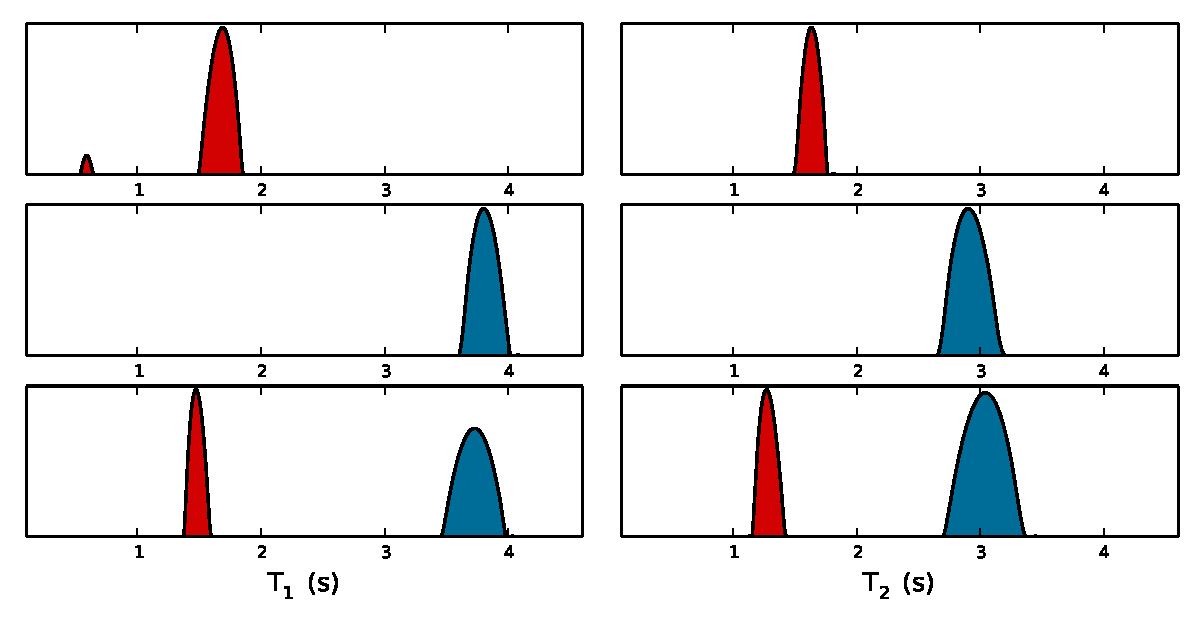
\includegraphics[width=\textwidth]{figures/relaxometry/decane-water-t1-t2-1d.eps}
    \caption{The 1-dimensional $\mathrm{T}_{1}$ and $\mathrm{T}_{2}$ pseudospectra of pure decane (top), pure water (center) and a decane/water mixture (bottom).}
    \label{fig:DecaneWater-1D-Data}
\end{figure}

As can be seen in Fig. \ref{fig:DecaneWater-1D-Data}, Laplace inversions of the data presented in Fig. \ref{fig:Decane-Water-Relaxation-Data} correctly pick out the number of components\footnote{The decane $\mathrm{T}_{1}$spectrum shows a small artifact peak, but this is likely due to an uncompensated offset in the instrument and is not a significant source of errors.} without any foreknowledge, and there is a clear separation between the two components.\cite{Song2007}

\begin{figure*}[h]
\centering
    \begin{subfigure}[t]{0.495\textwidth}
    \centering
    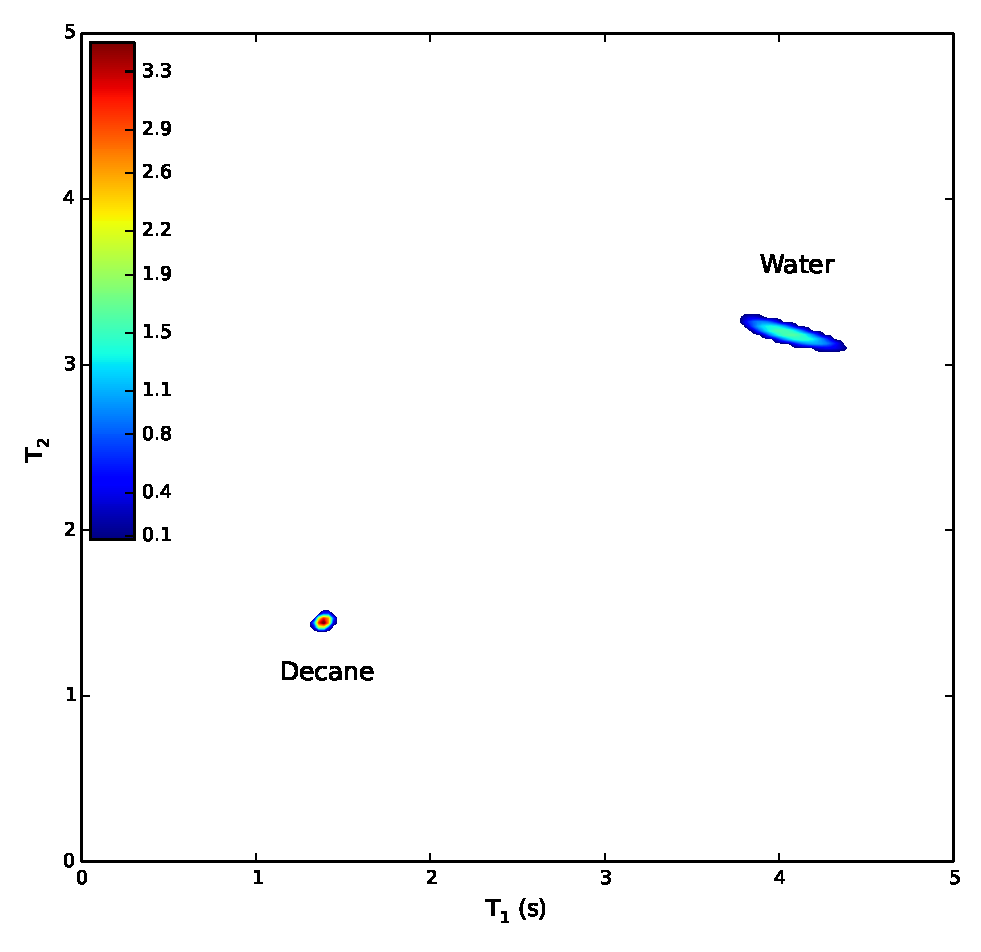
\includegraphics[width=\textwidth]{figures/relaxometry/decane-water-t1-t2.eps}
    \caption{}  
    \label{fig:DecaneWater-2D-T1T2-Data}
    \end{subfigure}
    \begin{subfigure}[t]{0.495\textwidth}
    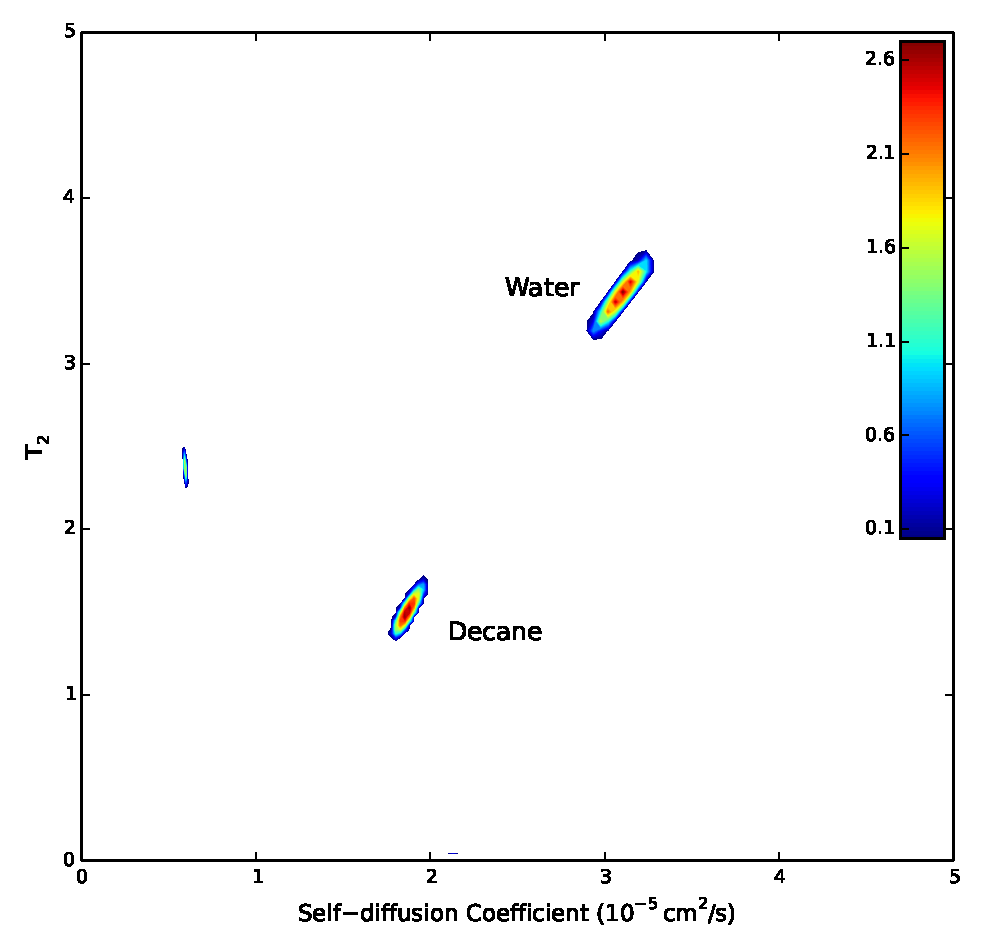
\includegraphics[width=\textwidth]{figures/relaxometry/decane-water-t2-d.eps}
    \caption{}  
    \label{fig:DecaneWater-2D-T2D-Data}
    \end{subfigure}
    \caption{$\mathrm{T}_{1}$-$\mathrm{T}_{2}$ (\ref{fig:DecaneWater-2D-T1T2-Data}) and $\mathrm{T}_{2}$-diffusion (\ref{fig:DecaneWater-2D-T2D-Data}) Laplace pseudospectra of decane and water. The extra peak in the $\mathrm{T}_{2}$-diffusion spectrum is an artifact of the inversion procedure used. The colors in the figure correspond to relative intensity, normalized to 100.}
    \label{fig:DecaneWater-2D-Data}
\end{figure*}

The same pulse sequences can also be used in two-dimensional correlation measurements to extract further information and help resolve close or broad components. Again using a decane/water mixture as the test sample, we performed $\mathrm{T}_{1}$-$\mathrm{T}_{2}$ and $\mathrm{T}_{2}$-diffusion correlation experiments, the resulting 2D pseudospectra are shown in Fig. \ref{fig:DecaneWater-2D-Data}.  As these data were acquired over a long time period (\unit[12-36]{h}), drift was a significant concern, and so experiments were acquired without active cooling to avoid potential temperature instabilities due to changes in the N$_2$ back pressure over the course of the day, and as such the results are a somewhat elevated temperature. For consistency, the data in Figs. \ref{fig:Decane-Water-Relaxation-Data}, \ref{fig:Decane-Water-Diffusion-Data} and \ref{fig:DecaneWater-1D-Data} were similarly performed without N$_2$ back pressure. Due to uncorrected drift over the course of the experiments, minor fast-relaxing artifacts appear in the $\mathrm{T}_{2}$-diffusion Laplace psuedospectrum; these artifacts do not significantly affect the results and are likely unique to this experimental configuration.

\section{Low Field Relaxation Dynamics}
\label{relaxometry.dynamics}
\begin{figure}[ht!!]
\centering
    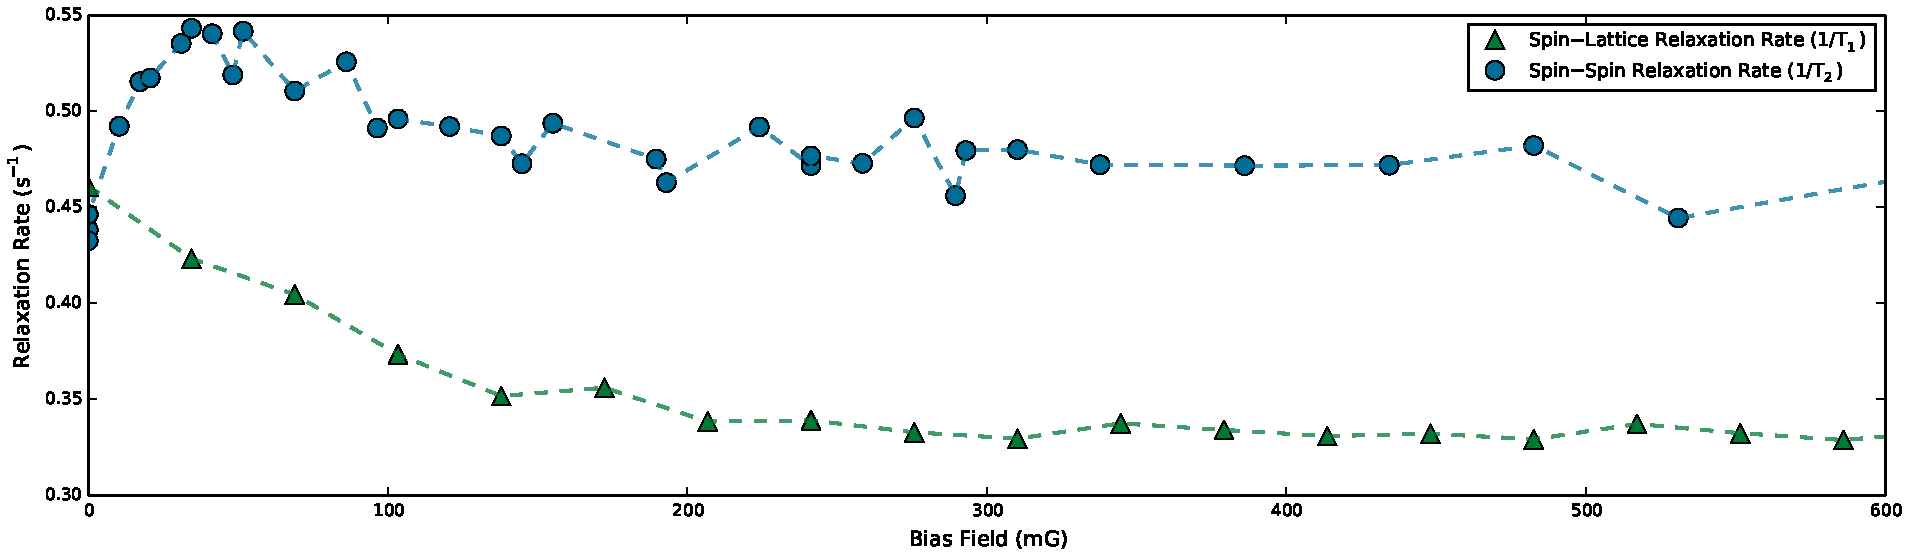
\includegraphics[width=0.95\textwidth]{figures/relaxometry/water-relaxation-t1t2.pdf}
    \caption{Measured relaxation rates (1/$\mathrm{T}_{1}$ and 1/$\mathrm{T}_{2}$) as a function of the bias offset field at \unit[36]{\degsym C}.}
    \label{fig:LowFieldRelaxation-WaterT1T2-Data}
\end{figure}

One significant advantage of performing our experiments in a field-cycled indirect dimension (as detailed in Sec. \ref{nmr.indirect}) is that the detection field can easily be changed without any recalibration. This allows us to use the field in which the experiment is performed as an additional dimension in the experiment. As a test of these capabilities, we measured the $\mathrm{T}_{1}$ and $\mathrm{T}_{2}$ of water as a function of field at very low fields (<\unit[1]{G}). We also made a cursory study of the effect of small magnetic fields on $\mathrm{T}_{2}$ relaxation of various hydrocarbon solvents.

The values measured here, having been acquired at an elevated temperature (\unit[36]{\degsym C}), are not directly comparable to the literature values, which were measured at room temperature, but the features of the data set are largely in agreement. At zero field there is no symmetry-breaking bias field, and as such there should be no distinction between $\mathrm{T}_{1}$ and $\mathrm{T}_{2}$, which is confirmed by the data presented in Fig. \ref{fig:LowFieldRelaxation-WaterT1T2-Data}. Below \unit[100]{mG}, we also observe the anomalously high relaxation rates first presented in \emph{Hartwig et al., 2011}\cite{Hartwig2011}.

\begin{figure}[ht!]
\centering
\begin{minipage}[t]{0.45\tw}
\centering
    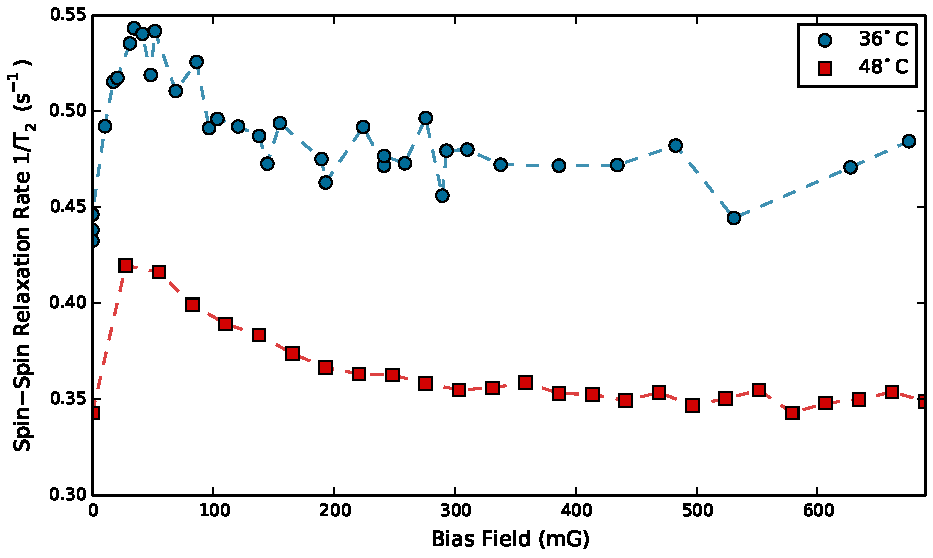
\includegraphics[width=\textwidth]{figures/relaxometry/water-relaxation-t2temp.pdf}
    \caption{The measured spin-spin relaxation rate (1/$\mathrm{T}_{2}$) as a function of field for two different temperatures, \unit[36]{\degsym C} and \unit[48]{\degsym C}}
    \label{fig:LowFieldRelaxation-WaterT2Temp-Data}
\end{minipage}
\hspace{0.01cm}
\begin{minipage}[t]{0.45\tw}
\centering
    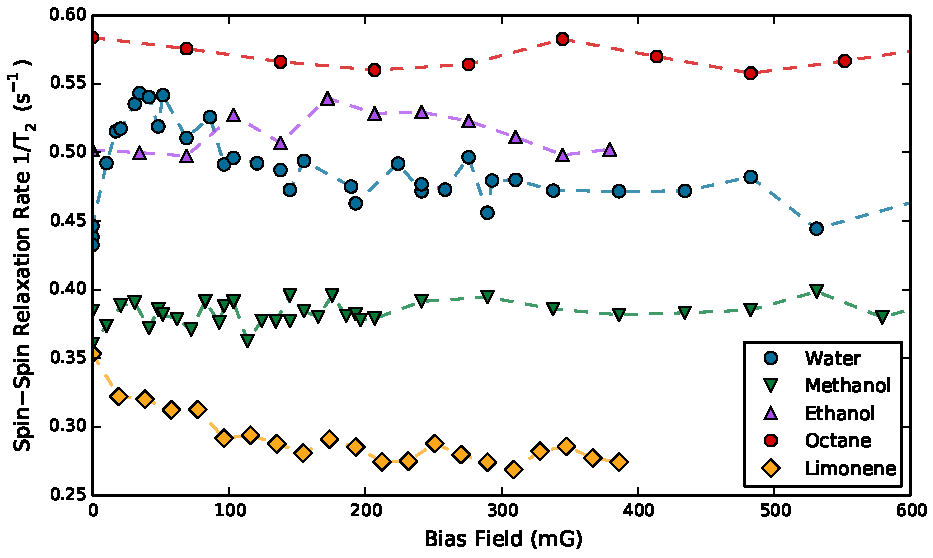
\includegraphics[width=\textwidth]{figures/relaxometry/solvent-relaxation-t2f.pdf}
    \caption{The measured spin-spin relaxation rate (1/$\mathrm{T}_{2}$) as a function of field for several hydrocarbon-based solvents at \unit[36]{\degsym C}}
    \label{fig:LowFieldRelaxation-Solvents-Data}
\end{minipage}
\end{figure}

As a general test for possible compounding of the effect of temperature and bias offset field on relaxation rates in water, we repeated the $\mathrm{T}_{2}$-field measurement without any dry N$_2$ flow cooling the sample, which raised the temperature to \unit[47]{\degsym C}. The data, shown in Fig. \ref{fig:LowFieldRelaxation-WaterT2Temp-Data}, scale roughly uniformly with the change in temperature, which is preliminary evidence against any compound temperature-field effects in low field water relaxation dynamics.

Finally, we performed a small survey of the effect of small magnetic fields on various hydrocarbon solvents, the results of which are presented in \ref{fig:LowFieldRelaxation-Solvents-Data}. There was not enough time to fully explore this space, and so only $\mathrm{T}_{2}$ data were acquired for a small number of solvents. A further exploration of this space could potentially be useful in identifying an ideal field in which to perform field-cycled NMR relaxometry in order to maximize contrast between sample components. In our experiments, $\mathrm{T}_{2}$ was measured to test whether anomalous low-field relaxation would be observed in other systems, particularly methanol and ethanol, but the $\mathrm{T}_{1}$ dynamics at low field would likely be a more generally useful data set; this is because $\mathrm{T}_{1}$ is generally measured in an indirect dimension anyway, using either inversion- or saturation-recovery pulse sequences, and it is easier to field cycle samples in an indirect dimension than to change the field in a direct dimension. 

\end{document}